\documentclass{article}
\usepackage[utf8]{inputenc}
\usepackage{algorithm}
\usepackage{algorithmic}
\usepackage{amsfonts}
\usepackage{amsmath}
\usepackage{amssymb}
\usepackage{amsthm}
\usepackage{bm}
\usepackage{bbm}
\usepackage{booktabs}
\usepackage{dsfont}
\usepackage{enumitem}
\usepackage{extarrows}
\usepackage{float} 
\usepackage{graphicx}
\usepackage{hyperref}
\usepackage{inconsolata}
\usepackage{listings}
\usepackage{makecell}
\usepackage{mathrsfs}
\usepackage{multicol}
\usepackage{multirow}
\usepackage{setspace}
\usepackage{subfigure} 
\usepackage{threeparttable}
\usepackage{tikz}
\usepackage{ulem}
\usetikzlibrary{decorations.markings}
\setitemize[1]{itemsep=0.8pt,partopsep=0.8pt,parsep=\parskip,topsep=0.8pt}
\DeclareMathAlphabet{\mathpzc}{OT1}{pzc}{m}{it}
%% Number of equations.
\numberwithin{equation}{section}
%% New symbols.
\newcommand{\rmb}{\mathrm{b}}
\newcommand{\e}{\mathrm{e}}
\newcommand{\E}{\mathbb{E}}
\newcommand{\ind}{\perp\!\!\!\perp}
\newcommand{\bfw}{\mathbf{w}}
\newcommand{\bbC}{\mathbb{C}}
\newcommand{\bbN}{\mathbb{N}}
\newcommand{\bbP}{\mathbb{P}}
\newcommand{\bbQ}{\mathbb{Q}}
\newcommand{\bbR}{\mathbb{R}}
\newcommand{\bbZ}{\mathbb{Z}}
\newcommand{\scr}{\mathscr}
\renewcommand{\cal}{\mathcal}
\newcommand{\loc}{\mathrm{loc}}
\newcommand{\ol}{\overline}
\newcommand{\wh}{\widehat}
\newcommand{\wt}{\widetilde}
\DeclareMathOperator{\id}{Id}
\DeclareMathOperator{\gr}{Gr}
\DeclareMathOperator{\tr}{tr}
\DeclareMathOperator{\cov}{Cov}
\DeclareMathOperator{\var}{Var}
\DeclareMathOperator{\supp}{supp}
\DeclareMathOperator{\diam}{diam}
\DeclareMathOperator{\re}{Re}
\DeclareMathOperator{\im}{Im}
\DeclareMathOperator{\res}{Res}
\DeclareMathOperator{\Log}{Log}
\DeclareMathOperator{\esssup}{ess\,sup}
\renewcommand{\d}{\mathrm{d}}

\renewcommand{\Im}{\mathrm{Im}}
\renewcommand{\i}{\mathrm{i}}
\renewcommand{\proofname}{\textit{Proof}}
\renewcommand*{\thesubfigure}{(\arabic{subfigure})}
\renewcommand{\baselinestretch}{1.18}

\theoremstyle{plain}
\newtheorem{theorem}{Theorem}[section]
\newtheorem{lemma}[theorem]{Lemma}
\newtheorem{proposition}[theorem]{Proposition}
\newtheorem{corollary}[theorem]{Corollary}
\newtheorem{example}[theorem]{Example}
\theoremstyle{definition}
\newtheorem{definition}[theorem]{Definition}
\newtheorem*{remark}{Remark}

\title{\bf Selected Topics in Complex Analysis}
\usepackage{geometry}
\geometry{a4paper, scale=0.80}
\author{\textsc{Jyunyi Liao}}
\date{}
\begin{document}
\maketitle
\tableofcontents
\newpage
\section{Preliminaries}
\subsection{Topology of the Complex Plane}
Before we proceed, we introduce some useful terminology in topology.
\begin{definition}
We use $\bbC$ to denote the complex plane $\{x+iy:x,y\in\bbR\}$.
\begin{itemize}
\item[(i)] Let $z_0\in\bbC$, and $r>0$. We use $B(z_0,r)$ to denote the \textit{open disc} of radius $r$ centered at $z_0$:
\begin{align*}
	B(z_0,r)=\left\{z\in\bbR:\vert z-z_0\vert<\delta\right\}.
\end{align*}
Any set $U\subset\bbC$ that contains an open disc centered at $z_0$ is called a \textit{neighborhood} of $z_0$.
\item[(ii)] A subset $U\subset\bbC$ is said to be \textit{open}, if for all $z\in U$, there exists $\delta>0$ such that $D(z,\delta)\subset U$. A subset $D\subset\bbC$ is said to be \textit{closed} if its complement $D^c=\bbC\backslash D$ is open. Particularly, the complex plane $\bbC$ and the empty set $\emptyset$ are both open and closed.
\item[(iii)] A point $z\in\bbC$ is said to be a \textit{limit point} (or an \textit{accumulation point}) of a set $E\subset\bbC$, if $$B(z,\delta)\cap E\backslash\{z\}\neq\emptyset$$ for all $\delta>0$. In other words, $z$ is a limit point of $E$ if each neighborhood of $z$ contains a point of $E$ that is not $z$. Note that $z$ is not required to be a point of $E$.
\item[(iv)] A point $z\in\bbC$ is said to be an \textit{interior point} of a set $E\subset\bbC$, if there exists $\delta>0$ such that $B(z,\delta)\subset E$. In other words, $z$ is an interior point of $E$ if $E$ is a neighborhood of $z$.
\item[(v)] The \textit{closure} of a set $E\subset\bbC$ is the set of all limit point of $E$, denoted by $\ol{E}$:
\begin{align*}
	\ol{E}=\left\{z\in E:\forall\delta>0,\ B(z,\delta)\cap E\backslash\{z\}\neq\emptyset\right\}.
\end{align*}
The \textit{interior} of a set $E\subset\bbC$ is the set of all interior point of $E$, denoted by $\mathring{E}$:
\begin{align*}
	\mathring{E}=\left\{z\in E:\exists\delta>0,\ B(z,\delta)\subset E\right\}.
\end{align*}
\item[(vi)] The \textit{boundary} of a set $E\subset\bbC$ is $\partial E=\ol{E}\cap\ol{E^c}$.
\item[(vii)] A set $K\subset\bbC$ is said to be \textit{compact}, if every open cover of $K$ has a finite subcover. In other words, for any collection of open sets $\{U_\alpha\}_{\alpha\in J}$ with $K\subset\bigcup_{\alpha\in J}U_\alpha$, there exist finitely many indices $\alpha_1,\cdots,\alpha_n\in J$ such that $K\subset\bigcup_{j=1}^n U_{\alpha_j}$.
\item[(viii)] A set $C\subset\bbC$ is said to be \textit{connected}, if there do not exist two disjoint nonempty open sets $A$ and $B$ such that $C\subset A\cup B$, and neither $A$ nor $B$ contains $C$. 
\item[(ix)] Given $z_1,z_2\in\bbC$, we use $[z_1,z_2]$ to denote the line segments on $\bbC$ with endpoints $z_1$ and $z_2$. A \textit{polygonal line} is a finite union of line segments of the form $[z_0,z_1]\cup[z_1,z_2]\cup\cdots\cup[z_{n-1},z_n]$. 
\item[(x)] If any two points of a set $E\subset\bbC$ can be connected by a polygonal line contained in $E$, then $E$ is said to be \textit{polygonally connected}.
\end{itemize}
\end{definition}
Since the complex plane $\bbC$ is homeomorphic to the Euclidean space $\bbR^2$, some standard results of the topology of Euclidean spaces follows.
\begin{proposition}\label{prop:1.2}
Let $E$ be a subset of $\bbC$.
\begin{itemize}
\item[(i)] $E$ is closed if and only if $E$ contains all its limit point.
\item[(ii)] The closure $\ol{E}$ is closed, and it is the minimal closed set that contains $E$. In other word, for any closed set $D\supset E$, we have $D\supset\ol{E}$.
\item[(iii)] The interior $\mathring{E}$ is open, and it is the maximal open set that is contained $E$. In other word, for any open set $U\subset E$, we have $U\subset\mathring{E}$.
\item[(iv)] $E$ is compact if and only if it is closed and bounded in $\bbC$.
\item[(v)] If $E$ is polygonally connected, then it is connected.
\item[(vi)] If $E$ is a connected open set, then $E$ is polygonally connected.
\end{itemize}
\end{proposition}
\begin{proof}
Here we only provide a proof of (vi), since it is related to our later discussion. Take $z_0\in E$. Let $A$ be the set of all points of $E$ that can be polygonally connected to $z_0$ in $E$, and let $B$ be the set of all points of $E$ that cannot be polygonally connected to $z_0$ in $E$. 

We claim that $A$ is an open set. For every $z\in A$, we can choose an open disc centered at $z$ and contained in $E$. Since $z$ is polygonally connected to $z_0$, so is every point in the open disc by joining a line segment connecting the point and the center $z$. Similarly, $B$ is also an open set.

Finally, we point out that, since $A$ contains $z_0$, and the connected set $E$ is a disjoint union of open sets $A$ and $B$, the set $B$ must be empty. Therefore, every point in $E$ is polygonally connected to $z_0$, and every two point in $E$ is polygonally connected by joining two polygonal lines intersecting at $z_0$.
\end{proof}

\paragraph{Remark.} According to this proof, we can even make our statement stronger. For any two points in a connected open domain $E$, they can be connected by a polygonal line, of which any two successive vertices represent the endpoints of a horizontal or vertical segment.


\paragraph{} To end this section, we see a useful application of polygonal connectedness. A complex-valued function $f:\bbC\to\bbC$ can be split into real and imaginary parts:
\begin{align*}
	f(z)=f(x+iy)=u(x,y)+iv(x,y),
\end{align*}
where $u,v$ are both real-valued functions on $\bbR^2$. 
\begin{proposition}
If the function $u(x,y)$ has partial derivatives $u_x$ and $u_y$ that vanish at every point of a connected open domain $U$, then $u$ is a constant in $U$.
\end{proposition}
\begin{proof}
Let $(x,y),(\wt x,\wt y)\in U$, so they can be connected by a polygonal path that is contained in $U$. Any two successive vertices of
the path represent the endpoints of a horizontal or vertical segment. Hence, by the Lagrange mean-value theorem for one real variable, the change in $u$ between these vertices is given by the value of a partial derivative of $u$ somewhere between the endpoints times the difference in the non-identical coordinates of the endpoints. Since, however, $u_x$ and $u_y$ vanish identically in $U$, the change in $u$ is 0 between each pair of successive vertices. Therefore $u(x,y)=u(\wt x,\wt y)$. 
\end{proof}

In complex analysis, we are often interested in the sets that have no disjoint parts and no holes that go completely through it. These sets are called simply connected sets. A formal definition is given below.
\begin{definition}[Simply connected domains]
Let $U\subset\bbC$ be a connected open set. If for each point $z_0\in U^c$ and each $\epsilon>0$, there exists a continuous mapping $\gamma:[0,\infty)\to\bbC$ such that (i) $d(\gamma(t),U^c)<\epsilon$ for all $t\geq 0$, (ii) $\gamma(0)=z_0$, and (iii) $\lim_{t\to\infty}\vert\gamma(t)\vert=\infty$, then $E$ is said to be \textit{simply connected}.
\end{definition}
\paragraph{Remark.} Let $R$ be a rectangle in $\bbC$. \textit{If $U$ is a simply connected open set, and $\partial R\subset U$, then $R\subset U$}. To verify this, assume $z_0\in R$ is not in $U$. Then any path $\gamma$ from $z_0$ to $\infty$ intersects $\partial R$ at some $\gamma(t)\in\partial R$. Since $\gamma(t)\in U$, there exists $B(\gamma(t),\delta)\subset U$, and $d\gamma(t)z,U^c)\geq\delta$. This contradicts (i)!

\newpage
\subsection{Differentiability and Holomorphy}
Similar to the derivative for real-valued functions, we can define the derivative for complex-valued functions $f:\bbC\to\bbC$, which is given by the limit
\begin{align}
	f^\prime(z)=\lim_{h\to 0}\frac{f(z+h)-f(z)}{h}.\label{complexdiff}
\end{align}
Note that in this definition, the quantity $h$ is complex. If the limit (\ref{complexdiff}) exists at some point $z\in\bbC$, we say that $f$ is \textit{(complex) differentiable} at $z$, and the limit is called the \textit{derivative} of $f$ at $z$.

\begin{theorem}[Cauchy-Riemann equation]
Let $f:\bbC\to\bbC$, and let $f(x+iy)=u(x,y)+iv(x,y)$, where $u$ and $v$ are real and imaginary parts of $f$, respectively. If $f$ is differentiable at $z\in\bbC$, then the partial derivatives $u_x,u_y,v_x,v_y$ exists at $z$, and they satisfy the Cauchy-Riemann equation:
\begin{align}
\begin{cases}
	u_x-v_y=0,\\
	v_x+u_y=0.
\end{cases}\label{cauchyriemann}
\end{align}
\end{theorem}
\begin{proof}
Fix any $z=x+iy\in\bbC$. Since $f$ is differentiable at $z$, the limit
\begin{align*}
	\lim_{h\to 0}\frac{f(z+h)-f(z)}{h}
\end{align*}
exists. We consider the limit along the real and imaginary directions:
\begin{align*}
	\lim_{\bbR\ni h\to 0}\frac{f(z+h)-f(z)}{h}=\lim_{\bbR\ni h\to 0}\frac{u(x+h,y)-u(x,y)+i\left(v(x+h,y)-v(x,y)\right)}{h}=u_x+iv_x,\\
	\lim_{\bbR\ni h\to 0}\frac{f(z+ih)-f(z)}{ih}=\lim_{\bbR\ni h\to 0}\frac{u(x,y+h)-u(x,y)+i\left(v(x,y+h)-v(x,y)\right)}{ih}=v_y-iu_y.
\end{align*}
The two limits should be equal, and the result follows.
\end{proof}

\paragraph{Remark.} The Cauchy-Riemann equation is not a sufficient condition for differentiability. Here consider
\begin{align*}
	f(z)=f(x,y)=\begin{cases}
		\displaystyle\frac{xy(x+iy)}{x^2+y^2}, &z\neq 0,\\
		0, &z=0.
	\end{cases}
\end{align*}
Since $f=0$ on coordinate axes, we have $u_x(0,0)+iv_x(0,0)=v_y(0,0)-iu_y(0,0)=0$, which is the Cauchy-Riemann equation at $z=0$. However, on the line $y=\alpha x$, we have
\begin{align*}
	\lim_{\bbR\ni x\to 0}\frac{f(x+i\alpha x)-f(0)}{x+i\alpha x}=\frac{\alpha}{1+\alpha^2},
\end{align*}
which depends on $\alpha$. Hence the limit at $z=0$ does not exist. In the next theorem, we provide a practical sufficient condition for differentiability.

\begin{theorem}
Let $f:\bbC\to\bbC$, and let $f(x+iy)=u(x,y)+iv(x,y)$, where $u$ and $v$ are real and imaginary parts of $f$, respectively. If the partial derivatives $u_x,u_y,v_x,v_y$ exist in a neighborhood of $z$ and are continuous at $z$, and they satisfy the Cauchy-Riemann equation (\ref{cauchyriemann}).
\end{theorem}
\begin{proof}
Let $z=x+iy\in\bbC$ and $h=\xi+i\eta\in\bbC$. We want to show that
\begin{align*}
	\lim_{h\to 0}\frac{f(z+h)-f(z)}{h}=u_x+iv_x
\end{align*}
We decompose the difference of $f$ as follows:
\begin{align*}
	f(z+h)-f(z)&=u(x+\xi,y+\eta)-u(x,y)+iv(x+\xi,y+\eta)-iv(x,y)
\end{align*}
By mean-value theorem, there exist $\theta_1,\theta_2,\theta_3,\theta_4\in(0,1)$ such that
\begin{align*}
	u(x+\xi,y+\eta)-u(x,y)&=u(x+\xi,y+\eta)-u(x+\xi,y)+u(x+\xi,y)-u(x,y)\\
	&=\eta u_y(x+\xi,y+\theta_1\eta)+\xi u_x(x+\theta_2\xi,y),\\
	v(x+\xi,y+\eta)-v(x,y)&=v(x+\xi,y+\eta)-v(x+\xi,y)+v(x+\xi,y)-v(x,y)\\
	&=\eta v_y(x+\xi,y+\theta_3\eta)+\xi v_x(x+\theta_4\xi,y).
\end{align*}
By continuity of partial derivatives,
\begin{align*}
	\frac{f(z+h)-f(z)}{h}&=\frac{\eta}{\xi+i\eta}\left[u_y(x+\xi,y+\theta_1\eta)+iv_y(x+\xi,y+\theta_3\eta)\right]+\frac{\xi}{\xi+i\eta}\left[u_x(x+\theta_2\xi,y)+iv_x(x+\theta_4\xi,y)\right]\\
	&=\frac{\eta}{\xi+i\eta}\left[u_y(x,y)+iv_y(x,y)+\epsilon_1\right]+\frac{\xi}{\xi+i\eta}\left[u_x(x,y)+iv_x(x,y)+\epsilon_2\right],
\end{align*}
where $\epsilon_1$ and $\epsilon_2$ are quantities converging to $0$ as $h\to 0$. By Cauchy-Riemann equation at $z=x+iy$,
\begin{align*}
	\frac{f(z+h)-f(z)}{h}&=\frac{i\eta}{\xi+i\eta}\left[iv_x(x,y)+ u_x(x,y)-i\epsilon_1\right]+\frac{\xi}{\xi+i\eta}\left[u_x(x,y)+iv_x(x,y)+\epsilon_2\right]\\
	&=u_x(x,y)+iv_x(x,y)+\frac{\eta\epsilon_1+\xi\epsilon_2}{\xi+i\eta},
\end{align*}
Since
\begin{align*}
	\left\vert\frac{\eta\epsilon_1+\xi\epsilon_2}{\xi+i\eta}\right\vert\leq\vert\epsilon_1\vert+\vert\epsilon_2\vert\to 0
\end{align*}
as $h\to0$, the result follows.
\end{proof}

To end this section, we introduce some useful definitions.
\begin{definition}
Let $z_0\in\bbC$ be a point, and let $U\subset\bbC$ be an open set. Let $f:\bbC\to\bbC$ be a complex function.
\begin{itemize}
\item[(i)] If $f$ is differentiable in a neighborhood of a point $z_0$, then $f$ is said to be \textit{holomorphic} at $z_0$;
\item[(ii)] If $f$ is everywhere differentiable in $U$, then $f$ is said to be \textit{holomorphic} in $U$;
\item[(iii)] If $f$ is holomorphic in $\bbC$, then $f$ is said to be \textit{entire}.
\end{itemize}
\end{definition}

\begin{proposition}
Let $f:U\to\bbC$ be a holomorphic function in an open connected region $U$. 
\begin{itemize}
	\item[(i)] Let $f=u+iv$. If $u$ is a constant in $D$, so is $f$.
	\item[(ii)] If $\vert f\vert$ is a constant in $D$, so is $f$.
\end{itemize}
\begin{proof}
(i) This result follows from Cauchy-Riemann equation and the polygonal connectedness of $U$.

(ii) Let $f=u+iv$. It suffices to consider the case $\vert f\vert=\sqrt{u^2+v^2}\equiv c>0$. By taking derivatives on both sides of $u^2+v^2\equiv c$ in $U$, we obtain
\begin{align*}
	uu_x+vv_x=0,\quad uu_y+vv_y=0.
\end{align*}
By applying the Cauchy-Riemann equation twice, we have
\begin{align*}
	0=u(uu_x+vv_x)=u^2u_x+uvv_x=u^2u_x-vuu_y=u^2u_x+v^2v_y=(u^2+v^2)u_x.
\end{align*}
Hence $u_x\equiv 0$ in $U$. Similarly, we can show $u_y\equiv 0$ in $U$. Then the result follows from (i).
\end{proof}
\end{proposition}

\subsection{Complex Power Series and Analyticity}
\paragraph{Analytic Polynomial.} A polynomial $P(x,y)$ is said to be an \textit{analytic polynomial}, if there exists complex numbers $c_0,c_1,\cdots,c_n\in\bbC$ such that
\begin{align*}
	P(x,y)=c_0+c_1(x+iy)+c_2(x+iy)^2 +\cdots + c_n(x+iy)^n.
\end{align*} 
We then say that $P$ is a polynomial in the complex variable $z\in\bbC$, and write
\begin{align*}
	P(z)=c_0+c_1z+c_2z^2+\cdots+c_nz^n.
\end{align*}
It is direct to verify that a polynomial $P(x,y)=u(x,y)+iv(x,y)$ is analytic if and only if it satisfies the Cauchy-Riemann equation (\ref{cauchyriemann}).

\paragraph{} A power series of $z$ is given by an ``infinite polynomial''.
\begin{definition}[Complex power series]
A power series in $z$ is an infinite series of the form
\begin{align*}
	f(z)=\sum_{n=0}^\infty c_nz^n,
\end{align*}
where $c_0,c_1,\cdots\in\bbC$.
\end{definition}

Naturally, we are interested in the domain where a power series converges.
\begin{theorem}\label{powercvg}
Suppose $\limsup_{n\to\infty}\vert c_n\vert^{1/n}=L$.
\begin{itemize}
\item[(i)] If $L=0$, the power series $\sum_{n=0}^\infty c_nz^n$ converges for all $z\in\bbC$. In this case, $R=\infty$ is called the radius of convergence of the power series.
\item[(ii)] If $L=\infty$, the power series $\sum_{n=0}^\infty c_nz^n$ converges if and only if $z=0$. In this case, $R=0$ is called the radius of convergence of the power series.
\item[(iii)] If $0<L<\infty$, set $R=\frac{1}{L}$. Then the power series $\sum_{n=0}^\infty c_kz^k$ converges for all $\vert z\vert<R$, and diverges for all $\vert z\vert>R$. In this case, $R$ is called the radius of convergence of the power series.
\item[(iv)] When the radius of convergence $R>0$, the power series $\sum_{n=0}^\infty c_nz^n$ converges uniformly on the closed disc $\ol{B(0,r)}$ for each $0<r<R$.
\end{itemize}
\end{theorem}
\begin{proof}
(i) When $L=0$, we have $\limsup_{n\to\infty}\vert c_n\vert^{1/n}\vert z\vert=0$ for all $z\in\bbC$. Hence for each $z\in\bbC$, there exists some
$N$ such that $\vert c_nz^n\vert<2^{-n}$ for all $n\geq N$. Therefore the series converges by Cauchy's criterion.

(ii) When $L=\infty$ and $z\neq 0$, we have $\vert c_n\vert^{1/n}>1/\vert z\vert$ for infinitely many $n\in\bbN$. Then the terms of the series do not approach $0$ as $n\to\infty$, and the series diverges.

(iii) Assume $0<L<\infty$, and $R=1/L$. If $\vert z\vert<R$, we set $\vert z\vert=R(1-2\epsilon)$ for some $\epsilon>0$. Then
\begin{align*}
	\limsup_{n\to\infty}\vert c_n\vert^{1/n}\vert z\vert<1-\epsilon,
\end{align*}
and we have $\vert c_nz^n\vert<(1-\epsilon)^n,\ n\geq N$ beginning from some $N$. On the other hand, when $\vert z\vert>R$, we have $\limsup_{n\to\infty}\vert c_n\vert^{1/n}\vert z\vert>1$, and there exists infinitely many terms greater than $1$ in the series.

(iv) The case $R=\infty$ is clear if we can prove the case $R<\infty$. When $R<\infty$, for all $\vert z\vert\leq r<R$, we have
\begin{align*}
	\limsup_{n\to\infty}\vert c_n\vert^{1/n}\vert z\vert\leq\frac{r}{R}< 1-\frac{R-r}{2R}:=1-\epsilon.
\end{align*}
Hence we have $\vert c_nz^n\vert<(1-\epsilon)^n,\ n\geq N$ beginning from some $N$. For $k\geq N$, the remainder $\sum_{n=k+1}^\infty c_nz^n$ is uniformly controlled by $(1-\epsilon)^k/\epsilon$ on $\ol{B(0,r)}$. Hence the convergence is uniform. 
\end{proof}

We can write the derivative of a power series into termwise differentiation.
\begin{theorem}\label{powerholo}
Let $f(z)=\sum_{n=0}^\infty c_nz^n$ be a power series with the radius $R>0$ of convergence. Then $f$ is holomorphic in $B(0,R)$, and
\begin{align*}
	f^\prime(z)=\sum_{n=1}^\infty nc_nz^{n-1},\quad\vert z\vert<R.
\end{align*}
Furthermore, the above series has the same radius of convergence as $f$.
\end{theorem}

The following corollary is easily obtained by applying Theorem \ref{powerholo} recursively.
\begin{corollary}
Let $f(z)=\sum_{n=0}^\infty c_nz^n$ be a power series with the radius $R>0$ of convergence. Then $f$ is infinitely differentiable in $B(0,R)$, and 
\begin{align*}
	c_n=\frac{f^{(n)}(0)}{n!},\quad\forall n\in\bbN_0.
\end{align*}
\end{corollary}

We now introduce the definition of analytic functions in the complex plane.
\begin{definition}[Analyticity]
Let $f:U\to\bbC$ be a complex function on an open set $U$, and let $z_0\in U$. The function $f$ is said to be \textit{analytic} at point $z_0$, if there exists complex coefficients $c_0,c_1,\cdots\in\bbC$ such that
\begin{align*}
	f(z)=\sum_{n=0}^\infty c_n(z-z_0)^n
\end{align*}
in a neighborhood of $z_0$. In other words, $f$ is analytic at $z_0$ if it equals a power series near $z_0$.
\end{definition}
\paragraph{Remark.} By definition, if $f$ is analytic at $z_0$, it is also holomorphic at $z_0$. In later discussion, we will show that the two properties are equivalent.

\begin{theorem}[Uniqueness theorem for power series]\label{pwsruniq}
We have the following result:
\begin{itemize}
\item[(i)] If a power series equals zero at all the points of a nonzero sequence $(z_k)_{k=1}^\infty$ that converges to zero, the power series is identically zero.
\item[(ii)] If two power series $\sum_{n=0}^\infty a_nz^n$ and $\sum_{n=0}^\infty b_nz^n$ converge and agree on a set of points with an accumulation point at the origin, then $a_n = b_n$ for all $n$.
\end{itemize}
\end{theorem}
\begin{proof}
(i) Let $f(z)=\sum_{n=0}^\infty c_nz^n$. By the continuity of $f$ at the origin, 
\begin{align*}
	c_0=f(0)=\lim_{z\to 0} f(z)=\lim_{k\to\infty} f(z_k)=0.
\end{align*}
Then $g(z)=\frac{f(z)}{z}=c_1+c_2z+c_3z^2+\cdots$ is also continuous at the origin, and 
\begin{align*}
	c_1=g(0)=\lim_{z\to 0}\frac{f(z)}{z}=\lim_{k\to\infty}\frac{f(z_k)}{z_k}=0.
\end{align*}
By induction, for all $n\in\bbN$,
\begin{align*}
	c_n=\lim_{z\to 0}\frac{f(z)}{z^n}=\lim_{k\to\infty}\frac{f(z_k)}{z_k^n}=0.
\end{align*}
(ii) We can reduce the set to a sequence of points since we can always choose a point $z_n$ from each neighborhood $B(0,n^{-1})$ of the origin. Then consider the series $\sum_{n=0}^\infty(b_n-a_n)z^n$ and apply (i).
\end{proof}

\newpage
\section{Cauchy's Integral Theorem and its Consequences}
\subsection{Complex Line Integral}
In this section, we deal with the integral on the complex plane $\bbC$.
\begin{definition}[Smooth curves]
Let $x=x(t)$ and $y=y(t)$ be continuous real-valued functions on $[a,b]$. If we use these equations as the real and imaginary parts in $z=x+iy$, we can parameterize the points $z$ on a curve $C$ by means of a complex-valued function of a real-variable $t$: 
$$C=\{z(t)=x(t)+iy(t),\ a\leq t\leq b\}.$$ 
\begin{itemize}
\item[(i)] The curve $C$ parameterized by $z(t)$ is said to be \textit{differentiable}, if both $x$ and $y$ are continuously differentiable on $[a,b]$. We define the derivative of $z(t)$ by
\begin{align*}
	z^\prime(t)=x^\prime(t)+iy^\prime(t),\quad a\leq t\leq b.
\end{align*}
Furthermore, if $z^\prime(t)\neq 0$ for all $a<t<b$, then $C$ is said to be \textit{smooth}.
\item[(ii)] The a curve $C$ is said to be \textit{piecewise smooth}, if $C$ can be obtained by joining finitely many smooth curves. Formally, if $C$ is piecewise smooth, we can find a partition $a=t_0<t_1<\cdots<t_n=b$ such that $z(t)$ is continuous on $[a,b]$, is continuously differentiable on each sub-interval $[t_{j-1},t_j]$, and $z^\prime(t)\neq 0$ except at finitely many points.
\item[(iii)] The curve $C$ is said to be simple if $z$ injective, i.e. $s\neq t$ implies $z(s)\neq z(t)$.
\item[(iv)] The curve $C$ is said to be \textit{closed} if $z(a)=z(b)$.
\item[(v)] A simple closed curve $C$ is said to be a \textit{contour} (or a \textit{Jordan curve}). By Jordan curve theorem, a contour always divide the complex plane $\bbC$ into two connected open components. One of these components is bounded and simply connected, called the \textit{interior of $C$}, and the other component is unbounded, called the \textit{exterior of $C$}. Furthermore, the contour $C$ is the boundary of each component.
\end{itemize}
\end{definition}

\begin{definition}[Complex integral]
Let $f(t)=u(t)+iv(t)$ be a continuous complex valued function of the real variable $a\leq t\leq b$, where $u$ and $v$ are both real-valued. Define
\begin{align*}
	\int_a^b f(t)\,dt=\int_a^b u(t)\,dt+i\int_a^b v(t)\,dt.
\end{align*}
Let $C$ be a smooth curve given by $z(t),\ a\leq t\leq b$, and suppose $f:\bbC\to\bbC$ is continuous at all the points $z(t)$. Then, the integral of $f$ along $C$ (or round $C$, if $C$ is a contour) is
\begin{align*}
	\int_C f(z)\,dz=\int_a^b f(z(t))\,z^\prime(t)\,dt.
\end{align*}
\end{definition}

\paragraph{Remark.} By this definition, the linearity of complex line integral follows from the real case. Furthermore, the value of the integral is independent of the particular parameterization. To see this, we consider two particular smooth curves
\begin{align*}
	C_1:z(t),\ a\leq t\leq b\quad and\quad C_2:\omega(t),\ c\leq t\leq d.
\end{align*}
We assume that there exists a bijective $C^1$-mapping $\lambda:[a,b]\to[c,d]$ such that $c=\lambda(a)$, $d=\lambda(b)$, $\lambda^\prime(t)>0$ for all $t\in[a,b]$, and $z(t)=\omega(\lambda(t))$. Then $C_1$ and $C_2$ are \textit{smoothly equivalent} in the complex plane $\bbC$, and
\begin{align*}
	\int_{C_1} f(z)\,dz=\int_a^b f(z(t))z^\prime(t)\,dt=\int_a^b f(\omega(\lambda(t)))\omega^\prime(\lambda(t))\lambda^\prime(t)\,dt\overset{s=\lambda(t)}{=}\int_c^d f(\omega(s))\omega^\prime(s)\,ds=\int_{C_2} f(z)\,dz.
\end{align*}

\paragraph{Change the direction.} The line integral depends not only on the set of points of the curve, but also the direction of the curve. Given a curve $C$ parameterized by $z(t),\ a\leq t\leq b$, the curve $-C$ along the opposite direction is given by $z(b+a-t),\ a\leq t\leq b$. Then
\begin{align*}
	\int_{-C} f(z)\,dz = \int_a^b f(z(b+a-t))\left(-z^\prime(b+a-t)\right)dt=-\int_a^b f(z(s))z^\prime(s)\,ds=-\int_C f(z)\,dz,
\end{align*}
where we change the variable $s=b+a-t$ in the second identity.

\paragraph{Estimation.} Now we aim to derive a bound for the complex line integral. Before we proceed, we point out that a smooth curve $C=\{z(t):a\leq t\leq b\}$ is \textit{rectifiable}, and its length is given by
\begin{align*}
	L=\int_C\vert dz\vert=\int_a^b\vert z^\prime(t)\vert\,dt=\sup_{a=t_0<t_1<\cdots<t_n=b}\sum_{j=1}^n\vert z(t_i)-z(t_{i-1})\vert.
\end{align*}
We will use this definition to estimate a complex integral.
\begin{lemma}
Let $F:[a,b]\to\bbC$ be a complex function that is continuous at each point of $C$. Then
\begin{align*}
	\left\vert\int_a^b F(t)\,dt\right\vert\leq\int_a^b\vert F(t)\vert\,dt.
\end{align*}
\end{lemma}
\begin{proof}
Assume that $\int_a^b F(z)\,dz=re^{i\theta}$, where $r=\left\vert\int_a^b F(z)\,dz\right\vert$ and $\theta\in[0,2\pi)$. Then
\begin{align*}
	r=\int_a^be^{-i\theta}F(t)\,dt=\int_a^b\re\left(e^{-i\theta}F(t)\right)dt\leq\int_a^b\left\vert e^{-i\theta}F(t)\right\vert dt=\int_a^b\vert F(t)\vert\,dt.
\end{align*}
Thus we complete the proof.
\end{proof}
\begin{theorem}[M-L formula]\label{mlformula}
Let $C=\{z(t):a\leq t\leq b\}$ be a piecewise smooth curve of length $L$. Let $f$ be a complex function that is continuous at each point of $C$, and $\vert f\vert\leq M$ on $C$. Then
\begin{align*}
	\left\vert\int_C f(z)\,dz\right\vert\leq ML.
\end{align*}
\end{theorem}
\begin{proof}
According to the previous lemma, we have
\begin{align*}
	\left\vert\int_C f(z)\,dz\right\vert=\left\vert\int_a^b f(z(t))z^\prime(t)\,dt\right\vert\leq\int_a^b\vert f(z(t))\vert\left\vert z^\prime(t)\right\vert dt\leq M\int_a^b\left\vert z^\prime(t)\right\vert dt=ML.
\end{align*}
Thus we complete the proof.
\end{proof}
\paragraph{Fundamental theorem of complex line integrals.} For complex functions, the Newton-Leibniz formula also holds. This formula is really helpful. It removes the dependence of the integral value on the integral path, so the integral value only relies on the initial and terminal points.
\begin{theorem}[Fundamental theorem of complex line integrals]\label{newtonleb}
Let $C=\{z(t):a\leq t\leq b\}$ be a piecewise smooth curve. Let $F$ be a complex function defined in an open set containing $C$. Suppose that $F$ is holomorphic at each point of $C$, and the derivative $f(z)=F^\prime(z)$ is continuous at each point of $C$. Then
\begin{align*}
	\int_C f(z)\,dz=F(z(b))-F(z(a)).
\end{align*}
\end{theorem}
\begin{proof}
Let $G(t)=F(z(t)),\ a\leq t\leq b$. By the chain rule, the derivative of $G$ is
\begin{align*}
	G^\prime(t)=\lim_{\bbR\ni h\to 0}\frac{G(t+h)-G(t)}{h}=\lim_{\bbR\ni h\to 0}\frac{F(z(t+h))-F(z(t))}{z(t+h)-z(t)}\cdot\frac{z(t+h)-z(t)}{h}=F^\prime(z(t))z^\prime(t).
\end{align*}
Then
\begin{align*}
	\int_C f(z)\,dz=\int_a^b F^\prime(z(t))z^\prime(t)\,dt=\int_a^b G^\prime(t)\,dt=G(b)-G(a)=F(z(b))-F(z(a)),
\end{align*}
where the third equality holds by apply Newton-Leibniz formula on both real and imaginary parts.
\end{proof}

\paragraph{Uniform Convergence.} In the real case, one can interchange the integral and the function limit when the function sequence to be integrated is uniformly convergent. This result also applies to the complex line integral. A function sequence $(f_n)$ \textit{converges uniformly} to $f$ on a set $U\subset\bbC$, if
\begin{align*}
	\lim_{n\to\infty}\sup_{z\in U}\vert f_n(z)-f(z)\vert = 0.
\end{align*}
We have the following theorem.
\begin{theorem}\label{unifconvergence}
Let $U$ be an open domain, and let $(f_n)$ be a sequence of continuous functions which converges uniformly on $U$. For any piecewise smooth curve $C=\{z(t):a\leq t\leq b\}$ in $U$,
\begin{align*}
	\lim_{n\to\infty}\int_C f_n(z)\,dz=\int_C\lim_{n\to\infty}f_n(z)\,dz.
\end{align*}
\end{theorem}
\begin{proof}
Let $f$ be the uniform limit of $(f_n)$ on $U$, which is also continuous. By M-L formula [Theorem \ref{mlformula}],
\begin{align*}
	\left\vert\int_C f(z)\,dz-\int_C f_n(z)\,dz\right\vert\leq\sup_{z\in U}\vert f(z)-f_n(z)\vert\int_C\vert dz\vert\to 0.
\end{align*}
Thus we complete the proof.
\end{proof}

\subsection{Cauchy-Goursat Theorem}
From now on, we assume that all the curves and contours we study are piecewise smooth. Unless otherwise specified, we also assume that all contour integrals are taken in the counterclockwise direction, which is consistent with the unit circle $\{e^{i\theta}:0\leq\theta\leq 2\pi\}$.

We study the contour integral of holomorphic functions in this section. Before we proceed, we first study a special case of the contour integral, where the contour is assumed to be the boundary of a rectangle.
\begin{lemma}\label{affinecontour}
Let $\Gamma$ be the boundary of a rectangle $R$. Let $f$ be an affine function defined in an open domain $U$ containing $R$, i.e. $f$ is of the form $f(z)=\alpha+\beta z$. Then
\begin{align*}
	\int_\Gamma f(z)\,dz=0.
\end{align*}
\end{lemma}
\begin{proof}
Note that $f$ is everywhere the derivative of an entire function $F(z)=\alpha z+\frac{1}{2}\beta z^2$, and that $\Gamma$ is a closed curve. Assume $\Gamma=\{z(t):a\leq t\leq b\}$, so $z(a)=z(b)$. The result immediately follows from Theorem \ref{newtonleb}.
\end{proof}

\begin{lemma}\label{recintegral}
Let $\Gamma$ be the boundary of a rectangle $R$. Let $f$ be a holomorphic function defined in an open domain $U$ containing $R$. Then
\begin{align*}
	\int_\Gamma f(z)\,dz=0.
\end{align*}
\end{lemma}
\begin{proof}
We write $I=\left\vert\int_\Gamma f(z)\,dz\right\vert$.To show that $I = 0$, we use the method of continued bisection. That is, we split the rectangle $R$ into four congruent subrectangles by bisecting each of the sides. We denote by $\Gamma_1,\Gamma_2,\Gamma_3,\Gamma_4$ the boundaries of the four rectangles. Since the integral on the interior lines cancels out when integrating along opposite directions, we have
\begin{align*}
\int_\Gamma f(z)\,dz=\sum_{i=1}^4\int_{\Gamma_i}f(z)\,dz.
\end{align*}
\begin{figure}[H]
\centering
\includegraphics[width=0.6\linewidth]{bisec.png}
\end{figure}
Hence for at least one $\Gamma_i,\ 1\leq i\leq 4$, denoted by $\Gamma^{(1)}$,
\begin{align*}
	\left\vert\int_{\Gamma^{(1)}}f(z)\,dz\right\vert\geq\frac{I}{4}.
\end{align*}
Let $R^{(1)}$ be the rectangle bounded by $\Gamma^{(1)}$. We repeat this procedure by dividing $R^{(n)}$ into four congruent subrectangles. Then we obtain a nested sequence
\begin{align*}
	R^{(1)}\supset R^{(2)}\supset R^{(3)}\supset\cdots
\end{align*}
with their boundaries $\Gamma^{(1)},\Gamma^{(2)},\Gamma^{(3)},\cdots$. This sequence satisfies $\diam R^{(n+1)}=\frac{1}{2}\diam R^{(n)}$, and
\begin{align}
	\left\vert\int_{\Gamma^{(n)}}f(z)\,dz\right\vert\geq\frac{I}{4^n}.\label{recintest1}
\end{align}
Take $z_0\in\bigcap_{n=1}^\infty R^{(n)}$, which is nonempty by the nested interval theorem. Since $f$ is holomorphic at $z_0$,
\begin{align*}
	\lim_{z\to z_0}\frac{f(z)-f(z_0)}{z-z_0}=f^\prime(z_0).
\end{align*}
By Lemma \ref{affinecontour}, we have
\begin{align*}
	\int_{\Gamma^{(n)}}f(z)\,dz&=\int_{\Gamma^{(n)}}\left(f(z_0)+f^\prime(z_0)(z-z_0)+\left(\frac{f(z)-f(z_0)}{z-z_0}-f^\prime(z_0)\right)(z-z_0)\right)dz\\
	&=\int_{\Gamma^{(n)}}\left(\frac{f(z)-f(z_0)}{z-z_0}-f^\prime(z_0)\right)(z-z_0)\,dz.
\end{align*}
We assume that the largest side of the original boundary $\Gamma$ has length $\ell$. Then
\begin{align*}
	\int_{\Gamma^{(n)}}\vert dz\vert\leq\frac{4\ell}{2^n},\quad and\quad \vert z-z_0\vert\leq\frac{\sqrt{2}\ell}{2^n},\ \ \forall z\in\Gamma^{(n)}.
\end{align*}
We fix $\epsilon>0$, and choose $N$ so that
\begin{align*}
	\vert z-z_0\vert\leq\frac{\sqrt{2}\ell}{2^N}\quad\Rightarrow\quad\left\vert\frac{f(z)-f(z_0)}{z-z_0}-f^\prime(z_0)\right\vert\leq\epsilon.
\end{align*}
Then for all $n\geq N$, by M-L formula [Theorem \ref{mlformula}],
\begin{align}
	\left\vert\int_{\Gamma^{(n)}}f(z)\,dz\right\vert\leq\frac{4\sqrt{2}\ell^2}{4^n}\epsilon.\label{recintest2}
\end{align}
Combining (\ref{recintest1}) and (\ref{recintest2}), we have
\begin{align*}
	I\leq 4\sqrt{2}\ell^2\epsilon.
\end{align*}
Since $\epsilon>0$ can be chosen arbitrarily small, we have $I=0$.
\end{proof}

We use this lemma to show that any holomorphic function is the derivative of another one.

\begin{theorem}[Integral theorem]\label{intthm}
Let $U$ be a simply connected open domain. If $f:U\to\bbC$ is a holomorphic function in $U$, then f is everywhere the derivative of another holomorphic function in $U$. That is,
there exists a holomorphic function $F:U\to\bbC$ such that $F^\prime(z) = f(z)$ for all $z\in U$.
\end{theorem}
\begin{proof}
We may assume without loss of generality that $0\in U$. Define $F(z)$ as
\begin{align*}
	F(z)=\int_{\Gamma(z)}f(\zeta)\,d\zeta,\quad z\in U
\end{align*}
where $\Gamma(z)$ is a polygonal line contained in $U$, starting from $0$ and terminating at $z$, and every line segment is either horizontal or vertical. In fact, the value of this integral is independent of the choice of the particular path $\Gamma(z)$, because the difference of this integral along any two such paths can be represented as a contour integral round the boundaries of finitely many rectangles contained in $U$ (because $U$ is simply connected). Since $f$ is holomorphic through these rectangles, by Lemma \ref{recintegral}, the boundary integral always cancels out.

Fix $z\in U$. For sufficiently small $\vert h\vert>0$, we have
\begin{align*}
	F(z+h)-F(z)=\int_z^{z+h} f(\zeta)\,d\zeta
\end{align*}
Where $\int_z^{z+h}$ is the line integral along the segments $[z,z+\re h]\,\cup\,[z+\re h,z+h]$. Note that the line integral along line segments $[z,z+\re h]\cup[z+\re h,z+h]$ is $h$, we have
\begin{align}
	\frac{F(z+h)-F(z)}{h}-f(z)=\frac{1}{h}\int_z^{z+h} \left(f(\zeta)-f(z)\right)d\zeta.\label{segintF}
\end{align}
We then fix $\epsilon>0$, and choose $\delta>0$ such that $\vert f(\zeta)-f(z)\vert<\epsilon$ for all $\vert\zeta-z\vert<\delta$. According to the M-L formula [Theorem \ref{mlformula}], whenever $\vert h\vert<\delta$,
\begin{align*}
	\left\vert\frac{1}{h}\int_z^{z+h} \left(f(\zeta)-f(z)\right)d\zeta\right\vert\leq\frac{1}{\vert h\vert}\cdot 2\vert h\vert\epsilon=2\epsilon.
\end{align*}
Since $\epsilon>0$ is arbitrarily chosen, \ref{segintF} converges to $0$ when $h\to 0$. Therefore $f(z)=F^\prime(z)$.
\end{proof}

This result immediately gives the Cauchy's integral theorem for holomorphic functions.
\begin{theorem}[Cauchy-Goursat]\label{cauchycontourint}
Let $f:U\to\bbC$ be a holomorphic function in a simply connected open domain $U$. Let $C=\{z(t):a\leq t\leq b\}$ be a piecewise smooth contour in $U$. Then
\begin{align*}
	\int_C f(z)\,dz=0.
\end{align*}
\end{theorem}
\begin{proof}
By integral theorem [Theorem \ref{intthm}], we can find a holomorphic function $F:U\to\bbR$ whose derivative is $f$ everywhere in $U$. Then
\begin{align*}
	\int_C f(z)\,dz=F(z(b))-F(z(a))
\end{align*}
by Theorem \ref{newtonleb}. Since $C$ is closed, $z(a)=z(b)$, and the value of the integral is $0$.
\end{proof}
\paragraph{Remark.} According to our proof, to cancel out a contour integral, we only require that $f$ is the derivative of a  holomorphic function inside a simply connected open domain containing the contour $C$.

\begin{theorem}[Deformation principle]\label{deform}
Let $C_1$ and $C_2$ be contours, with $C_2$ lying wholly inside $C_1$, and suppose that $f$ is 
holomorphic in an open domain containing the closed domain between $C_1$ and $C_2$. Then 
\begin{align*}
	\int_{C_1} f(z)\,dz=\int_{C_2} f(z)\,dz.
\end{align*}
\end{theorem}
\begin{figure}[H]
	\centering
	\includegraphics[width=0.70\linewidth]{deform.png}
\end{figure}
\begin{proof}
We join $C_1$ and $C_2$ by two segments $[z_{11},z_{21}]$ and $[z_{22},z_{12}]$, as is shown in the figure. Then we obtain two contours on the upper domain $D_1$ and lower domain $D_2$, respectively, and the integrals of $f$ round these two contours are both $0$. We add up these two integrals, of which the part on the segments is canceled out:
\begin{align*}
	\int_{\partial D_1}f(z)\,dz+\int_{\partial D_2}f(z)\,dz=\int_{C_1}f(z)\,dz+\int_{-C_2}f(z)\,dz=0.
\end{align*}
In the last display, changing the direction of $-C_2$ and rearranging complete our proof.
\end{proof}
\paragraph{Remark.} In the deformation principle, we require $f$ to be holomorphic near the inner contour $C_2$, but we allow $f$ to be not holomorphic inside the inner contour.

\subsection{Cauchy's Integral Formula}
\paragraph{An important integral.} To begin this section, we first compute an important contour integral
\begin{align*}
	\int_C (z-z_0)^n\,dz,
\end{align*}
where $C$ is a piecewise smooth contour going around a fixed point $z_0\in\bbC$, and $n\in\bbZ$.
\begin{itemize}
\item\textit{Case I: $n\geq 0$.} In this case, $(z-z_0)^n$ is an analytic polynomial, which is entire. Then the value of the integral is $0$ by Cauchy-Goursat theorem [Theorem \ref{cauchycontourint}].
\item\textit{Case II: $n=-1$.} We use the deformation principle to compute this integral. Since $\frac{1}{z-z_0}$ is holomorphic on the whole complex plane $\bbC$ except at $z_0$, we choose a circle $\partial B(z_0,\epsilon)$ that is lying wholly inside $C$, which is parameterized by $\{z_0+\epsilon e^{i\theta}:0\leq\theta\leq 2\pi\}$:
\begin{align*}
	\int_C\frac{dz}{z-z_0}=\int_{\partial B(z_0,\epsilon)}\frac{dz}{z-z_0}=\int_0^{2\pi}\frac{i\epsilon e^{i\theta}d\theta}{\epsilon e^{i\theta}}=2\pi i.
\end{align*}
\item\textit{Case II: $n\leq -2$.} In this case, $(z-z_0)^n$ is the derivative of the function $\frac{(z-z_0)^{n+1}}{n+1}$, which is holomorphic on the whole on the whole complex plane $\bbC$ except at $z_0$. Since $C$ is closed, the value of the integral is $0$ by the fundamental theorem of complex line integral [Theorem \ref{newtonleb}].
\end{itemize}
We then summarize our result below:
\begin{align*}
	\int_C(z-z_0)^n\,dz=\begin{cases}
		0, & n\neq -1,\\
		2\pi i, & n=-1.
	\end{cases}
\end{align*}
The Cauchy's integral formula is motivated by this example.
\begin{theorem}[Cauchy's integral formula]\label{cauchyintformula}
Let $f:U\to\bbC$ be a holomorphic function in a simply connected open domain $U$. Let $C$ be any piecewise smooth contour in $U$ that goes around some fixed point $z_0\in U$. Then
\begin{align}
	f(z_0)=\frac{1}{2\pi i}\int_C\frac{f(z)}{z-z_0}\,dz.\label{cauchyintegral}
\end{align}
\end{theorem}
\begin{proof}
Since $\frac{f(z)}{z-z_0}$ is holomorphic in $U\backslash\{z_0\}$, by the deformation principle [Theorem \ref{deform}], we may change $C$ to any circle $\partial B(z_0,\epsilon)$ of radius $\epsilon>0$ and centered at $z_0$:
\begin{align*}
	\int_C\frac{f(z)}{z-z_0}\,dz&=\int_{\partial B(z_0,\epsilon)}\frac{f(z)}{z-z_0}\,dz\\
	&=\int_{\partial B(z_0,\epsilon)}\frac{f(z_0)+f^\prime(z_0)(z-z_0)+\left(f(z)-f(z_0)-f^\prime(z_0)(z-z_0)\right)}{z-z_0}\,dz\\
	&=\underbrace{\int_{\partial B(z_0,\epsilon)}\frac{f(z_0)}{z-z_0}\,dz}_{=\,2\pi i f(z_0)}+\underbrace{\int_{\partial B(z_0,\epsilon)}f^\prime(z_0)\,dz}_{=\,0}+\underbrace{\int_{\partial B(z_0,\epsilon)}\left(\frac{f(z)-f(z_0)}{z-z_0}-f^\prime(z_0)\right)dz}_{remainder}.
\end{align*}
By M-L formula [Theorem \ref{mlformula}], the remainder satisfies
\begin{align*}
	\left\vert\int_C\frac{f(z)}{z-z_0}\,dz-2\pi i f(z_0)\right\vert=\left\vert\int_{\partial B(z_0,\epsilon)}\left(\frac{f(z)-f(z_0)}{z-z_0}-f^\prime(z_0)\right)dz\right\vert\leq2\pi\epsilon\sup_{\vert z-z_0\vert\leq\epsilon}\left\vert \frac{f(z)-f(z_0)}{z-z_0}-f^\prime(z_0)\right\vert.
\end{align*}
The remainder can be dominated by arbitrarily small quantity as $\epsilon\to 0$. Then (\ref{cauchyintegral}) follows.
\end{proof}

We have similar results for higher order derivatives.

\begin{theorem}[Generalized Cauchy's integral formula]\label{generalcauchy}
Let $f:U\to\bbC$ be a holomorphic function in a simply connected open domain $U$. Then $f$ is infinitely differentiable in $U$, and 
\begin{align}
	f^{(n)}(z_0)=\frac{n!}{2\pi i}\int_C\frac{f(z)}{(z-z_0)^{n+1}}\,dz,\label{generalizedcauchyint}
\end{align}
where $C$ is any piecewise smooth contour in $U$ that goes around some fixed point $z_0\in U$.
\end{theorem}
\begin{proof}
Since $U$ is open, we can find an open disc $B(z_0,\epsilon)\subset U$. We fix $C$ to be its boundary $\vert z-z_0\vert=\epsilon$. Then for all $z$ with $\vert z-z_0\vert=\epsilon$ and $\omega\in B(z_0,\frac{\epsilon}{2})$, we have the expansion
\begin{align}
	\frac{1}{z-\omega}=\frac{1}{(z-z_0)\left(1-\frac{\omega-z_0}{z-z_0}\right)}=\sum_{n=0}^\infty\frac{(\omega-z_0)^n}{(z-z_0)^{n+1}}.\label{geometricexp}
\end{align}
This series converges uniformly on $B(z_0,\frac{\epsilon}{2})$, since for all $n\in\bbN$,
\begin{align*}
	\left\vert\sum_{n=N+1}^\infty\frac{(\omega-z_0)^n}{(z-z_0)^{n+1}}\right\vert<\frac{1}{2^N\epsilon},\quad\forall\omega\in B\left(z_0,\frac{\epsilon}{2}\right).
\end{align*}
Then we apply Theorem \ref{unifconvergence} to interchange the infinite sum and the integration:
\begin{align*}
	f(\omega)=\frac{1}{2\pi i}\int_C\frac{f(z)}{z-\omega}\,dz&=\frac{1}{2\pi i}\int_C\sum_{n=0}^\infty\frac{f(z)(\omega-z_0)^n}{(z-z_0)^{n+1}}\,dz\\
	&=\sum_{n=0}^\infty\left(\frac{1}{2\pi i}\int_C\frac{f(z)}{(z-z_0)^{n+1}}\,dz\right)(\omega-z_0)^n,\quad\omega\in B\left(z_0,\frac{\epsilon}{2}\right).
\end{align*}
Therefore, $f$ can be written into a power series in a neighborhood $B(z_0,\frac{\epsilon}{2})$. Furthermore, the coefficients are in fact independent of our choice of $C$ by the deformation principle, since $C$ lies in $U$ and goes around $z_0$. Hence $f$ is infinitely differentiable in this neighborhood, and
\begin{align*}
	f^{(k)}(\omega)=\sum_{n=k}^\infty\left(\frac{n(n-1)\cdots(n-k+1)}{2\pi i}\int_C\frac{f(z)}{(z-z_0)^{n+1}}\,dz\right)(\omega-z_0)^{n-k},\quad\omega\in B\left(z_0,\frac{\epsilon}{2}\right).
\end{align*}
Taking $\omega=z_0$, we obtain (\ref{generalizedcauchyint}), which completes the proof.
\end{proof}

The proof above also establishes the analyticity of holomorphic functions. We can even modify our result to make it a little stronger.
\begin{corollary}
Let $f:U\to\bbC$ be a holomorphic function in a simply connected open domain $U$. Then $f$ is analytic in $U$. Furthermore, for each $z_0\in U$, $f$ can be represented as the local Taylor series near $z_0$:
\begin{align*}
	f(\omega)=\sum_{n=0}^\infty\frac{f^{(n)}(z_0)}{n!}(\omega-z_0)^n=\sum_{n=0}^\infty\left(\frac{1}{2\pi i}\int_C\frac{f(z)}{(z-z_0)^{n+1}}\,dz\right)(\omega-z_0)^n,\quad \omega\in B(z_0,\epsilon)\subset U,
\end{align*}
where $B(z_0,\epsilon)$ is the largest open disc centered at $z_0$ and contained in $U$.
\end{corollary}
\begin{proof}
Since $\omega\in B(z_0,\epsilon)$, there exists $\theta>0$ such that $\omega\in B(z_0,(1-\theta)\epsilon)$. Then we fix $C$ to be the circle $\vert z-z_0\vert=(1-\frac{\theta}{2})\epsilon$. With this choice, the power series (\ref{geometricexp}) still converges uniformly on $B(z_0,(1-\theta)\epsilon)$, and the remainder totally follows from the previous proof.
\end{proof}

\paragraph{Remark.} If $f:\bbC\to\bbC$ is entire, then $f$ is globally equal to its Taylor series at any point $z_0\in\bbC$.

\subsection{Liouville's Theorem and the Fundamental Theorem of Algebra}
\begin{theorem}[Liouville's Theorem]\label{liouvillethm}
A bounded entire function is a constant.
\end{theorem}
\begin{proof}
Let $f:\bbC\to\bbC$ be a entire function bounded by some $M>0$. For each  $z_1,z_2\in\bbC$, we take any circle $C=\{z:\vert z\vert=R\}$ with $R>\max\{\vert z_1\vert,\vert z_2\vert\}$. By Cauchy's integral formula,
\begin{align*}
	f(z_1)-f(z_2)=\frac{1}{2\pi i}\int_C\frac{f(z)}{z-z_1}\,dz-\frac{1}{2\pi i}\int_C\frac{f(z)}{z-z_2}\,dz=\frac{1}{2\pi i}\int_C\frac{f(z)(z_2-z_1)}{(z-z_1)(z-z_2)}\,dz.
\end{align*}
By M-L formula [Theorem \ref{mlformula}],
\begin{align*}
	\left\vert f(z_1)-f(z_2)\right\vert=\frac{1}{2\pi}\left\vert\int_C\frac{f(z)(z_2-z_1)}{(z-z_1)(z-z_2)}\,dz\right\vert\leq\frac{MR\left\vert z_2-z_1\right\vert}{(R-\vert z_1\vert)(R-\vert z_2\vert)}\to 0,\quad R\to\infty.
\end{align*}
Hence $f(z_1)=f(z_2)$ for all $z_1,z_2\in\bbC$, and $f$ is a constant on $\bbC$.
\end{proof}

\begin{theorem}[Extended Liouville's Theorem]\label{extliouvillethm}
If $f:\bbC\to\bbC$ is an entire function, and if for some integer $k\geq 0$, $f$ grows no faster than $\vert z\vert^k$, that is, there exist constants $A,B>0$ such that
\begin{align*}
	\vert f(z)\vert\leq A+B\vert z\vert^k,\quad\forall z\in\bbC,
\end{align*}
then $f$ is a polynomial of degree at most $k$.
\end{theorem}
\begin{proof}
The case $k=0$ is the original Liouville theorem, and we use induction to prove the general case. We define a new function $g:\bbC\to\bbC$ as follows:
\begin{align*}
	g(z)=\begin{cases}
		\frac{f(z)-f(0)}{z},\quad z\neq 0\\
		f^\prime(0),\quad z=0
	\end{cases}\quad\Rightarrow\quad g(z)=\sum_{n=1}^\infty\frac{f^{(n)}(0)}{n!}z^{k-1},\quad z\in\bbC.
\end{align*}
Clearly, $g$ is also an entire function. We pick any $R>0$. Then $g(z)$ is bounded in the compact disc $\vert z\vert\leq R$, and its absolute value grows no faster than $\vert z\vert^{k-1}$ as $z\to\infty$. Hence there exists $C,D>0$ such that
\begin{align*}
	\vert g(z)\vert\leq C+D\vert z\vert^{k-1}.
\end{align*}
According to the induction hypothesis, $g$ is polynomial of degree at most $k-1$. Therefore $f$ is a polynomial of degree at most $k$.
\end{proof}

We then use Liouville's theorem to prove the fundamental theorem of algebra.
\begin{lemma}\label{lemmafundalge}
Every non-constant polynomial with complex coefficients has a zero in $\bbC$.
\end{lemma}
\begin{proof}
Let $P(z)$ be a non-constant polynomial. If $P(z)$ has no zero in $\bbC$, then $\frac{1}{P(z)}$ is an entire function. Since $P(z)$ is non-constant, $P(z)\to\infty$ as $z\to\infty$, and $\frac{1}{P(z)}$ is bounded in $\bbC$. By Liouville's theorem, $\frac{1}{P(z)}$ is a constant, and so is $P(z)$, which is a contradiction!
\end{proof}

\begin{theorem}[Fundamental theorem of algebra]\label{fundalge}
If $P(z)$ is a polynomial of degree $n\geq 1$ with complex coefficients, then there exist complex numbers $A$ and $z_1,\cdots,z_n$ such that
\begin{align*}
	P(z)=A(z-z_1)(z-z_2)\cdots(z-z_n),\quad z\in\bbC.
\end{align*}
\end{theorem}
\begin{proof}
The case $n=1$ is clear, and the general case follows by induction. By the previous lemma, any polynomial $P(z)$ of degree $n$ has a zero $z_n\in\bbC$, and the function $Q(z)=\frac{P(z)}{z-z_n}$ grows no faster than $\vert z\vert^{n-1}$. By the extended Liouville's theorem, $Q(z)$ is a polynomial of degree $k-1$, and the result follows.
\end{proof}

\paragraph{Remark.} According to the fundamental algebra, we can write a polynomial $P(z)$ of degree $n$ to the form
\begin{align*}
	P(z)=A(z-z_1)^{m_1}(z-z_2)^{m_2}\cdots(z-z_k)^{m_k},
\end{align*}
where $z_1,z_2,\cdots,z_k\in\bbC$ are zeroes of $P(z)$ and are mutually distinct, and $m_1,\cdots,m_k$ are positive integers such that $m_1+\cdots+m_k=n$. The number $m_j$ is called the \textit{multiplicity} of the zero $z_j$. It is easy to see that $z_j$ is a zero of multiplicity $m_j$ if and only if
\begin{align}
	P(z_j)=P^\prime(z_j)=P^{\prime\prime}(z_j)=\cdots=P^{(m_j-1)}(z_j)=0,\quad P^{(m_j)}(z_j)\neq 0.\label{charmulti}
\end{align}
\paragraph{Factorization of polynomials with real coefficients.} We let $P(z)$ be a polynomial of degree $n$ with real coefficients. In this case, we have $P(\ol{z})=\ol{P(z)}$ for all $z\in\bbC$. Consequently, if $\omega\in\bbC$ is a zero of $P(z)$, so is $\ol{\omega}$. Furthermore, the conjugate zeroes have the same multiplicity by the condition (\ref{charmulti}). Therefore, there exists an integer $k\leq\frac{n}{2}$, non-real zeroes $\omega_1,\omega_2,\cdots,\omega_k\in\bbC$ and real zeroes $c_1,\cdots,c_{n-2k}\in\bbR$ such that
\begin{align*}
	P(z)=A(z-\omega_1)(z-\ol{\omega_1})(z-\omega_2)(z-\ol{\omega_2})\cdots(z-\omega_k)(z-\ol{\omega_k})(z-c_1)(z-c_2)\cdots(z-c_{n-2k}),
\end{align*}
Note that $(z-\omega_j)(z-\ol{\omega_j})$ is a quadratic polynomial with real coefficients:
\begin{align*}
	(z-\omega_j)(z-\ol{\omega_j})=z^2-\alpha_jz+\beta_j,\quad where\ \ \alpha_j=2\re\omega_j\ \ and\ \ \beta_j=\vert\omega_j\vert^2.
\end{align*}
Therefore, we have the following factorization of $P(z)$:
\begin{align*}
	P(z)=A\prod_{j=1}^k(z^2-\alpha_jz+\beta_j)\prod_{p=1}^{n-2k}(z-c_p),
\end{align*}
which consists of only linear and quadratic polynomials with real coefficients.

\paragraph{} We finally introduce a result concerning both the zeroes of a polynomial and of its derivative.

\begin{theorem}[Gauss-Lucas theorem]\label{gausslucas}
The zeroes of the derivative of any polynomial lie within the convex hull of the zeroes of the polynomial.
\end{theorem}
\begin{proof}
Let $P(z)$ be a polynomial of degree $n$ with zeroes $z_1,\cdots,z_n\in\bbC$. Then
\begin{align*}
	\frac{P^\prime(z)}{P(z)}=\frac{1}{z-z_1}+\frac{1}{z-z_2}+\cdots+\frac{1}{z-z_n},\quad\forall z\notin\{z_1,z_2,\cdots,z_n\}.
\end{align*}
Assume $\omega\in\bbC$ is a zero of $P^\prime(z)$. We may assume $\omega\in\{z_1,\cdots,z_n\}$, otherwise the result is clear. Then
\begin{align*}
	0=\ol{\left(\frac{P^\prime(\omega)}{P(\omega)}\right)}=\frac{\omega-z_1}{\vert \omega-z_1\vert^2}+\frac{\omega-z_2}{\vert \omega-z_2\vert^2}+\cdots+\frac{\omega-z_n}{\vert \omega-z_n\vert^2}.
\end{align*}
Hence
\begin{align*}
	\omega=\sum_{j=1}^n\lambda_j z_j,\quad where\ \ \lambda_j=\frac{\vert\omega-z_j\vert^{-2}}{\sum_{k=1}^n\vert\omega-z_k\vert^{-2}}>0,\ \ and\ \ \lambda_1+\cdots+\lambda_n=1.
\end{align*}
Then we conclude the proof.
\end{proof}
\paragraph{Remark.} By induction, for a polynomial $P(z)$ of degree $n$, the zeroes of the derivative $P^{(k)}(z)$ of any order $k=1,2,\cdots,n-1$ lie in the convex hull of the zeroes of $P(z)$.

\subsection{The Converse of Cauchy's Integral Theorem: Morera's Theorem}
The Cauchy's theorem asserts that the integral of any holomorphic function in a simple connected open domain round any contour inside the domain is zero. The following result, due to Morera, gives a converse statement.
\begin{theorem}[Morera's theorem]\label{morera}
Let $f:U\to\bbR$ be a continuous function on an open set $U$. If
\begin{align*}
	\int_C f(z)\,dz=0
\end{align*}
for all contours $C$ in $U$, then $f$ is holomorphic in $U$.
\end{theorem}
\begin{proof}
We fix $z_0\in U$, and choose an open disc $B(z_0,\delta)\subset U$. We then define the primitive
\begin{align*}
	F(z)=\int_{z_0}^z f(\zeta)\,d\zeta,
\end{align*}
where $\int_{z_0}^z$ denote the integral along the path $[z_0,z_0+\re(z-z_0)]\cup[z_0+\re(z-z_0),z]$. Like in the proof of Theorem \ref{intthm}, we consider a difference quotient of $F$ and that fact that $\int_\Gamma f(z)\,dz=0$ around any rectangle in $B(z_0,\delta)$, we may conclude that
\begin{align*}
	\frac{F(z+h)-F(z)}{h}-f(z)=\frac{1}{h}\int_{z}^{z+h}(f(\zeta)-f(z))d\zeta\to 0,\quad as\ \ h\to 0.
\end{align*}
Hence $F$ is holomorphic in $B(z_0,\delta)$, and $f=F^\prime$, which can be represented by a power series in $B(z_0,\delta)$, is holomorphic at $z_0$. Finally, since $z_0\in U$ is arbitrary, $f$ is holomorphic in $U$.
\end{proof}
\paragraph{Remark.} We can make the condition slightly weaker by letting $C$ to be any rectangular boundary inside $U$ with
sides parallel to the real and imaginary axes.

\paragraph{Compact convergence.} In some cases, we may concern whether the limit of a sequence of holomorphic functions is holomorphic. To answer this question, we need to introduce a new convergence mode. Let $(f_n)$ be a sequence of functions defined on a topological space $U$. We say that $(f_n)$ \textit{converges compactly to} $f$, if $f_n\to f$ uniformly on each compact subset $K$ of $U$. That is,
\begin{align*}
	\lim_{n\to\infty}\sup_{z\in K}\vert f_n(z)-f(z)\vert = 0,\quad\forall\  compact\ K\subset U.
\end{align*}

\begin{theorem}\label{compactholoconvg}
Let $(f_n)$ be a sequence of holomorphic functions in an open domain $U$ such that $f_n\to f$ compactly. Then $f$ is also holomorphic in $U$.
\end{theorem}
\begin{proof}
For each point $z_0$, $f$ is the uniform limit of the sequence $(f_n)$ on a compact disc $\ol{B(z_0,\delta)}$ about $z_0$. Hence $f$ is continuous in $U$. Furthermore, for any rectangular boundary $\Gamma\subset U$, since $\Gamma$ is compact, $f_n$ converges uniformly to $f$ on $\Gamma$. By Theorem \ref{unifconvergence},
\begin{align*}
	\int_\Gamma f(z)\,dz=\int_\Gamma\lim_{n\to\infty}f(z)\,dz=\lim_{n\to\infty}\int_\Gamma f(z)\,dz=0.
\end{align*}
Hence, by Morera’s theorem, $f$ is holomorphic in $U$.
\end{proof}

\begin{theorem}\label{segmentext}
Suppose $f$ is a continuous function in an open set $U$, and $f$ is holomorphic there except possibly at the
points of a line segment $L$. Then $f$ is holomorphic throughout $U$.
\end{theorem}
\begin{proof}
We may assume that the line segment $L$ lies on the real axis. Otherwise,  our proof applies to the function $g(z)=f(T^{-1}z)$, where $Tz=\frac{z-z_0}{z_1-z_0}$ is a linear transformation that maps any segment $[z_0,z_1]$ to the compact interval $[0,1]\subset\bbR$, and the holomorphy of $f$ in $U$ is equivalent to the holomorphy of $g$ in $TU$.

Since holomorphy is a local property, we may also assume that $U$ is an open disc. We prove that $\int_\Gamma f(z)\,dz=0$ for any rectangular boundary $\Gamma\subset U$  with
sides parallel to the real and imaginary axes.
\begin{itemize}
\item[(i)] When $L$ does not coincide the rectangular bounded by $\Gamma$, we have $\int_\Gamma f(z)\,dz$ by Cauchy-Goursat theorem.
\item[(ii)] When $L$ coincides with the bottom (top) side of $\Gamma$, we slightly shift up (down) the bottom (top) side by a small quantity $\epsilon>0$ and get a boundary $\Gamma_\epsilon$, which reduces to case (i). By boundedness and uniform continuity of $f$ on compact sets,
\begin{align*}
	\lim_{\epsilon\to 0}\left(\int_\epsilon^0 f(a+iy)\,dy+\int_a^b f(x+i\epsilon)\,dx+\int_0^\epsilon f(b+iy)\,dy\right)=0+\int_a^b f(x)\,dx+0=\int_a^b f(x)\,dx.
\end{align*}
for all $[a,b]\subset U$. Then
\begin{align*}
	\int_\Gamma f(z)\,dz=\lim_{\epsilon\to 0}\int_{\Gamma_\epsilon} f(z)\,dz=0.
\end{align*}
\item[(iii)] When $L$ is surrounded by $\Gamma$, split $\Gamma$ by the real line to $\Gamma_1$ and $\Gamma_2$. Then the integral of $\Gamma_1$ and $\Gamma_2$ reduces to the case (ii), and
\begin{align*}
	\int_{\Gamma}f(z)\,dz=\int_{\Gamma_1}f(z)\,dz+\int_{\Gamma_2}f(z)\,dz=0.
\end{align*}
\end{itemize}
Finally, by Morera's theorem, $f$ is holomorphic in $U$.
\end{proof}

\begin{theorem}[Schwarz Reflection Principle]
Suppose $f$ is holomorphic in a simply connected open domain $U$ that is contained in either the upper or lower half plane and whose boundary contains a segment $[a,b]$ on the real axis, and suppose
$f(z)\in\bbR$ for real $z$. Then we can define a holomorphic extension $g$ of $f$ to the domain $U\cup (a,b)\cup U^*$ that is symmetric with respect to the real axis by setting
\begin{align*}
	g(z)=\begin{cases}
		f(z),\ &z\in U\cup (a,b),\\
		\ol{f(\ol{z})}, & z\in U^*,
	\end{cases}
\end{align*}
where $U^*=\{\ol{z}:z\in U\}$.
\end{theorem}
\begin{proof}
If $z\in U^*$, we choose a small quantity $h$ with $z+h\in U^*$, then
\begin{align*}
	\lim_{h\to 0}\frac{g(z+h)-g(z)}{h}=\lim_{h\to 0}\frac{\ol{f(\ol{z}+\ol{h})-f(\ol{z})}}{h}=\lim_{h\to 0}\ol{\left[\frac{f(\ol{z}+\ol{h})-f(\ol{z})}{\ol{h}}\right]}=\ol{f^\prime(\ol{z})}.
\end{align*}
Hence $g$ is holomorphic both in $U$ and $U^*$. Since $f(z)\in\bbR$ for all real $z$, the function $f$ is continuous in the domain $U\cup (a,b)\cup U^*$. Then $f$ is also holomorphic in this domain by employing Theorem \ref{segmentext}.
\end{proof}
\begin{figure}[H]
\centering
\includegraphics[width=0.52\linewidth]{reflection.png}
\end{figure}
\newpage
\section{Singularities of Analytic Functions and Calculus of Residues}
\subsection{Branch Cuts}
\paragraph{Motivation.} We consider the logarithm function and the root function in a complex plane. Given a complex number $re^{i\theta}$, the solutions of the equation $e^z=re^{i\theta}$ are
\begin{align*}
	z=\log r+ i(\theta+2k\pi),\quad where\ k\in\bbZ,
\end{align*}
and the solutions of the equation $z^n=re^{i\theta}$ ($n=2,3,\cdots$) are
\begin{align*}
	z=r^{1/n}e^{i\frac{\theta+2k\pi}{n}},\quad where\ k=0,1,\cdots,n-1.
\end{align*}
These functions are multi-valued in the complex case, which map a number $z\in\bbC$ to a subset of $\bbC$. The difficulty comes from the fact that $z\mapsto e^z$ and $z\mapsto z^n$ are no longer bijective. In the last two cases, each $k$ correspond to a \textit{branch} of the multi-valued function. 

A \textit{branch cut} is a curve in the complex plane such that it is possible to define a single analytic branch of a multi-valued function on the plane minus that curve. 

\begin{definition}
Let $U$ be a simply connected open domain. A function $f:U\to\bbC$ is said to be an \textit{analytic branch of $\log(z)$}, if
\begin{itemize}
\item[(i)] $f$ is analytic in $U$, and
\item[(ii)] $f$ is an inverse of the exponential function there, i.e. $e^{f(z)}=z$.
\end{itemize}
\end{definition}
\paragraph{Remark.} When $z\in\bbC\backslash\{0\}$, the \textit{principal value} of $\log z$ is chosen to be the logarithm whose imaginary part lies in the interval $(-\pi,\pi]$, called the \textit{principle argument of $z$}, written $\mathrm{Arg}(z)$:
\begin{align*}
	\Log(z)=\log\vert z\vert + i\,\mathrm{Arg}(z),\quad z\in\bbC\backslash\{0\}.
\end{align*}
We choose the branch cut to be $(-\infty,0]$. On the simply connected open domain $U=\bbC\backslash(-\infty,0]$, the principal logarithm $z\mapsto\Log(z)$ is continuous, because both the modulus $\vert z+h\vert-\vert z\vert$ and the principal argument $\mathrm{Arg}(z+h)-\mathrm{Arg}(z)$ changes little within a small region $\vert h\vert<\epsilon$ for fixed $z\in U$. Then 
\begin{align*}
	\lim_{h\to 0}\frac{\Log(z+h)-\Log(z)}{h}=\left(\lim_{h\to 0}\frac{e^{\Log(z+h)}-e^{\Log(z)}}{\Log(z+h)-\Log(z)}\right)^{-1}=e^{-\Log(z)}=\frac{1}{z}.
\end{align*}
Therefore $\Log(z)$ is analytic in $\bbC\backslash(-\infty,0]$. This is a useful analytical branch of $\log(z)$.

\begin{theorem}
Let $U\subset\bbC$ be a simply connected domain such that $0\notin U$. We choose $z_0\in U$, fix a value of $\log z_0$ and define
\begin{align*}
	f(z)=\log z_0+\int_{z_0}^z\frac{d\zeta}{\zeta}.
\end{align*}
Then $f$ is an analytic branch of $\log(z)$ in $U$.
\end{theorem}
\begin{proof}
Since $1/\zeta$ is a holomorphic function of $\zeta$ in the simply connected open domain $U$, by Theorem \ref{intthm}, it is the derivative of some primitive holomorphic function in $U$, and the integral along any two paths from $z_0$ to $z$ has the same value. Then $f^\prime(z)=z^{-1}$ on $U$, and $f$ is holomorphic, hence analytic.

Now we consider the function $g(z)=ze^{-f(z)}$. Since $g^\prime(z)=e^{-f(z)}-zf^\prime(z)e^{-f(z)}=0$, the function $g$ is a constant in $U$, and $g(z)=g(z_0)=z_0e^{-f(z_0)}=1$. Hence $e^{f(z)}=z$, completing the proof.
\end{proof}

\paragraph{Remark.} The principal logarithm $z\mapsto\Log(z)$ corresponds to $z_0=1,\log 1=0$ and $U=\bbC\backslash(-\infty,0]$.

\subsection{Isolated Singularities}
In this section, we study the behavior of an analytic function in the neighborhood of an isolated singularity. We call a set of the form $U\backslash\{z_0\}$ a \textit{deleted neighborhood} of $z_0$, where $U$ is a neighborhood of $z_0$.
\begin{definition}
A function $f$ is said to have an \textit{isolated singularity} at $z_0$ if $f$ is holomorphic in a deleted neighborhood $U\backslash\{z_0\}$, but is not holomorphic at $z_0$.
\end{definition}
\paragraph{Remark.} According to Theorem \ref{segmentext}, $f$ must be \textit{discontinuous} at an isolated singularity.

\begin{definition}[Classification of isolated singularities]\label{singclass}
Assume that $f$ has a singularity at $z_0$. 
\begin{itemize}
\item[(i)] If there exists a function $g$ such that $f(z)=g(z)$ for all $z$ in some deleted neighborhood of $z_0$, we say $f$ has a \textit{removable singularity} at $z_0$.
\item[(ii)] If there exists analytic functions $A(z)$ and $B(z)$ such that $A(z_0)\neq 0$, $B(z_0)=0$ and $f(z)=\frac{A(z)}{B(z)}$ for all $z$ in some deleted neighborhood of $z_0$, we say $f$ has a \textit{pole} at $z_0$.

In addition, if $B(z)$ has a zero of multiplicity $k$ at $z_0$, the pole at $z_0$ is said to be \textit{of order $k$}. A pole of order 1 (resp. 2, 3) is called a simple (resp. double, triple) pole.
\item[(iii)] If f has neither a removable singularity nor a pole at $z_0$, we say $f$ has an \textit{essential singularity} at $z_0$.
\end{itemize}
\end{definition}

Now we discuss the properties of each class of singularity.
\begin{theorem}[Riemann’s principle of removable singularities]\label{removesing}
If $f$ has an isolated singularity at $z_0$ and if $\lim_{z\to z_0}(z-z_0) f(z)=0$, then the singularity is removable.
\end{theorem}
\begin{proof}
Define the function $h(z)=(z-z_0)f(z)$ in an appropriate deleted neighborhood of $z_0$, which is also analytic. If we add a continuous extension $h(z_0)=0$, by Theorem \ref{segmentext}, $h$ is also analytic at $z_0$. Then the function $g(z)=\frac{h(z)}{z-z_0}$ is analytic at $z_0$ and agrees with $f$ in a deleted neighborhood of $f$.
\end{proof}

\paragraph{Remark.} According to this theorem, if $f$ is bounded in a deleted neighborhood of an isolated singularity, then the singularity
is removable.

\begin{theorem}\label{polesing}
If $f$ has an isolated singularity at $z_0$ and if there exists a positive integer $k$ such that 
$$\lim_{z\to z_0}(z-z_0)^k f(z)\neq 0,\quad but\quad \lim_{z\to z_0}(z-z_0)^{k+1} f(z)=0$$ 
then the singularity at $z_0$ is a pole of order $k$.
\end{theorem}
\begin{proof}
We set $g(z)=(z-z_0)^{k+1}f(z)$ in an appropriate deleted neighborhood of $z_0$, and set $g(z_0)=0$. By Theorem \ref{segmentext}, $g$ is continuous and analytic at $z_0$. Likewise, the function $A(z)=\frac{g(z)}{z-z_0}=(z-z_0)^kf(z)$ is also analytic at $z_0$, and $A(z_0)\neq 0$ by hypothesis. Then we conclude the proof by setting $B(z)=(z-z_0)^k$ in the previous Definition \ref{singclass}(ii) of poles.
\end{proof}

\paragraph{Remark.} Combining Theorems \ref{removesing} and \ref{polesing}, we conclude that $f(z)$ has a pole of order $k$ at $z_0$ if and only if $(z-z_0)^kf(z)$ has a removable singularity at $z_0$.

\begin{theorem}[Casorati-Weierstrass Theorem]
If $f$ has an essential singularity at $z_0$ and if $D=U\backslash\{z_0\}$ is a deleted neighborhood of $z_0$, then the range $R=\{f(z):z\in D\}$ is dense in the complex plane.
\end{theorem}
\begin{proof}
Argue by contradiction. If there exists some open disc $B(\omega,\delta)$ not intersecting $R$, then $\vert f(z)-\omega\vert\geq\delta$, and $\frac{1}{\vert f(z)-\omega\vert}\leq\frac{1}{\delta}$ throughout $D$. By Riemann's principle of removable singularities, $\frac{1}{f(z)-\omega}$ has at worst a removable singularity at $z_0$, and $\frac{1}{f(z)-\omega}=g(z)$ on $D$ for some $g$ that is analytic at $z_0$. Consequently, we have $f(z)=\omega+\frac{1}{g(z)}$ near $z_0$. Therefore, $f$ has either a removable singularity (if $g(z_0)\neq 0$) or a pole (if $g(z_0)=0$) at $z_0$, contradicting the fact that $f$ has an essential singularity at $z_0$!
\end{proof}

\subsection{Laurent Series}
In the previous sections, we see that an analytic function in an open disc can be represented there by its Taylor series. For analytic functions in an \textit{annulus} $\{z\in\bbC:R_1<\vert z\vert<R_2\}$, we have a similar representation, which is in the form of a two-sided power series, which is called the \textit{Laurent series}.
\begin{theorem}
The series $f(z)=\sum_{n=-\infty}^\infty c_nz^n$ is convergent in the domain
\begin{align*}
	D=\left\{z\in\bbC:\vert z\vert<R_2\ and\ \vert z\vert>R_1\right\},
\end{align*}
where
\begin{align*}
	R_2=\left(\limsup_{n\to\infty}\vert c_n\vert^{1/n}\right)^{-1},\quad and\quad R_1=\limsup_{n\to\infty}\vert c_{-n}\vert^{1/n}.
\end{align*}
If $R_1<R_2$, $D=\{z\in\bbC:R_1<\vert z\vert<R_2\}$ is an annulus and $f$ is analytic in $D$.
\end{theorem}
\begin{proof}
Define power series $g(z)=\sum_{n=1}^\infty c_{-n}z^n$, and $f_2(z)=\sum_{n=0}^\infty c_nz^n$. By Theorem \ref{powercvg}, $g$ is convergent in the domain $\{z\in\bbC:\vert z\vert<1/R_1\}$, and $f_2$ is convergent in the domain $\{z\in\bbC:\vert z\vert<R_2\}$ are convergent. Furthermore, by Theorem \ref{powerholo}, they are both analytic in their respective domains. Let $f_1(z)=g(1/z)$, which is convergent and analytic in the domain $\{z\in\bbC:\vert z\vert>R_1\}$. Hence $f=f_1+f_2$ is convergent in $D$, and is analytic when $D$ is nonempty.
\end{proof}

\begin{theorem}
If $f$ is analytic in the annulus $D=\{z\in\bbC:R_1<\vert z\vert<R_2\}$, then $f$ has an expansion of the following form throughout $D$:
\begin{align}
	f(z)=\sum_{n=-\infty}^\infty c_nz^n.\label{laurentexp}
\end{align}
Furthermore, in this form, the coefficients $c_n$ are uniquely given by
\begin{align*}
	c_n=\frac{1}{2\pi i}\int_C\frac{f(z)}{z^{n+1}}\,dz,\ \ n\in\bbZ,
\end{align*}
where $C$ is any circle in $D$ centered at $0$. This expansion is called the \textit{Laurent series} of $f$ about $0$.
\end{theorem}
\begin{proof}
Choose $R_1<r_1<r_2<R_2$, and let $C_1$ and $C_2$ be the circles centered at $0$ of radii $r_1$ and $r_2$, respectively. Fix $z\in D$ with $r_1<\vert z\vert<r_2$. Since $f$ is analytic in $D$, so is the function $g(\omega)=\frac{f(\omega)-f(z)}{\omega-z}$ with $g(z)=f^\prime(z)$. By the deformation principle [Theorem \ref{deform}],
\begin{align}
	\int_{C_1}\frac{f(\omega)-f(z)}{\omega-z}\,d\omega=\int_{C_2}\frac{f(\omega)-f(z)}{\omega-z}\,d\omega,\quad z\in D.\label{laurentdeform}
\end{align}
Since $z$ lies inside $C_2$ and outside $C_1$,
\begin{align*}
	\int_{C_1}\frac{f(z)}{\omega-z}=0,\quad \int_{C_2}\frac{f(z)}{\omega-z}=2\pi i f(z).
\end{align*}
Therefore, we rearrange (\ref{laurentdeform}) and then use the power series $\frac{1}{1-t}=\sum_{n=0}^\infty t^n,\ \vert t\vert<1$:
\begin{align*}
	2\pi i f(z)&=\int_{C_2}\frac{f(\omega)}{\omega-z}\,d\omega-\int_{C_1}\frac{f(\omega)}{\omega-z}\,d\omega=\int_{C_2}\frac{f(\omega)}{\omega\left(1-\frac{z}{\omega}\right)}\,d\omega+\int_{C_1}\frac{f(\omega)}{z\left(1-\frac{\omega}{z}\right)}\,d\omega\\
	&=\int_{C_2}\sum_{n=0}^\infty f(\omega)\frac{z^n}{\omega^{n+1}}\,d\omega+\int_{C_1}\sum_{n=0}^\infty f(\omega)\frac{\omega^n}{z^{n+1}}\,d\omega.
\end{align*}
Note that $\sum_{n=0}^\infty f(\omega)\frac{z^n}{\omega^{n+1}}$ converges uniformly on the circle $C_2$, and $\sum_{n=0}^\infty f(\omega)\frac{\omega^n}{z^{n+1}}$ converges uniformly on the circle $C_1$. Therefore, we interchange the infinite sum and the integral by Theorem \ref{unifconvergence}:
\begin{align*}
	2\pi i f(z)=\sum_{n=0}^\infty\left(\int_{C_2}\frac{f(\omega)}{\omega^{n+1}}\,d\omega\right) z^n + \sum_{n=0}^\infty\left(\int_{C_1}\omega^nf(\omega)\,d\omega\right)\frac{1}{z^{n+1}}.
\end{align*}
Again, by the deformation principle, we can switch the integral paths $C_1$ and $C_2$ to any circle $C$ in $D$ centered at $0$ without changing the integral value:
\begin{align*}
	2\pi i f(z)=\sum_{n=-\infty}^\infty\left(\int_C\frac{f(\omega)}{\omega^{n+1}}\,d\omega\right)z^n.
\end{align*}
This ensures the existence of the expansion in form (\ref{laurentexp}). It remains to prove the uniqueness of this expansion. If the expansion $f(z)=\sum_{n=-\infty}^\infty c_nz^n$ converges in $D$, it converges uniformly on any circle $C$ lying in $D$ centered at $0$. Hence for all $k\in\bbZ$,
\begin{align*}
	\int_C\frac{f(z)}{z^{k+1}}\,dz=\sum_{n=-\infty}^\infty c_n\left(\int_C z^{n-k-1}\,dz\right)=2c_k\pi\i,
\end{align*}
where all terms in the infinite sum vanish except $n-k-1=-1$. This proves uniqueness.
\end{proof}
\paragraph{Remark.} For any point $z_0\in\bbC$, if $f$ is analytic in the annulus $D=\{z\in\bbC:R_1<\vert z-z_0\vert<R_2\}$, we can apply the previous result to the function $g(z)=f(z+z_0)$. This gives the Laurent series of $f$ about $z_0$:
\begin{align*}
	f(z)=\sum_{n=-\infty}^\infty c_n(z-z_0)^n,\quad R_1<\vert z\vert<R_2,
\end{align*}
where the coefficients are
\begin{align*}
	c_n=\frac{1}{2\pi i}\int_C\frac{f(z)}{(z-z_0)^{n+1}}\,dz,\quad n\in\bbZ,
\end{align*}
and $C=\partial B(z_0,R)$ is any circle of radius $R_1<R<R_2$ centered at $z_0$. Furthermore, an isolated singularity at $z_0$ corresponds to case of $R_1=0$. We formally state the result below.

\begin{corollary}
If $f$ have an isolated singularity at $z_0$, then $f$ equals to its Laurent series
\begin{align*}
	f(z)=\sum_{n=-\infty}^\infty c_n(z-z_0)^n=\sum_{n=-\infty}^\infty\left(\frac{1}{2\pi i}\int_C\frac{f(z)}{(z-z_0)^{n+1}}\,dz\right)(z-z_0)^n
\end{align*}
in some deleted neighborhood $0<\vert z-z_0\vert<\delta$ of $z_0$. 
\end{corollary}

\paragraph{Terminology.} The series $$f_a(z)=\sum_{n=0}^\infty c_n(z-z_0)^n$$ is called the \textit{analytic part of $f$ at $z_0$}.
The series $$f_p(z)=\sum_{n=1}^{\infty}\frac{c_{-n}}{(z-z_0)^n}$$ is called the \textit{principal part of $f$ at $z_0$}. We can use the principle part of the Laurent series to determine the class of isolated singularities.

\begin{theorem}\label{laurentsingularity}
Suppose $f$ has an isolated singularity at $z_0$, and the Laurent series of $f$ about $z_0$ is
\begin{align*}
	f(z)=\sum_{n=-\infty}^\infty c_n(z-z_0)^n,\quad 0<\vert z-z_0\vert<\delta.
\end{align*}
\begin{itemize}
\item[(i)] If $f$ has an isolated singularity at $z_0$, all the coefficients of the principle part are zero. 
\item[(ii)] If $f$ has a pole of order $k$ at $z_0$, then $c_{-k}\neq 0$ and $c_{-N}=0$ for all $N>k$. 
\item[(iii)] If $f$ has an essential singularity at $z_0$, then there are infinitely many nonzero terms in its principal part.
\end{itemize}
\end{theorem}
\begin{proof}
(i) If $f$ has an isolated singularity at $z_0$, then there exists a one-point modification $g$ of $f$ in an appropriate neighborhood of $z_0$, and $g$ is analytic at $z_0$. By the uniqueness argument, the Laurent series of $f$ about $z_0$ equals the Taylor series of $g$ at $z_0$.

(ii) If $f$ has a pole of order $k$ at $z_0$, there exists an analytic function $A(z)$ such that $f(z)=\frac{A(z)}{(z-z_0)^k}$ in an appropriate deleted neighborhood of $z_0$ and such that $A(z_0)\neq 0$. The result follows by plugging in the Taylor series of $A(z)$ at $z_0$ and uniqueness of the Laurent series.

(iii) If $f$ had an essential singularity at $z_0$, and there were only finitely many nonzero terms in its principal part, then $(z-z_0)^N f(z)$ would be analytic for large enough $N$ and hence $f$ would have either a removable singularity or a pole at $z_0$.
\end{proof}

We can use the Laurent series to derive a partial fraction decomposition of any rational function.
\begin{theorem}[Partial fraction decomposition]
Any proper rational function
\begin{align*}
	R(z)=\frac{P(z)}{Q(z)}=\frac{P(z)}{(z-z_1)^{k_1}(z-z_2)^{k_2}\cdots(z-z_n)^{k_n}},
\end{align*}
where $P$ and $Q$ are polynomials with $\deg P<\deg Q$ and $z_1,\cdots,z_n\in\bbC$ are mutually distinct, can be written as a sum of polynomials in $\frac{1}{z-z_j}$, where $j=1,2,\cdots,n$. That is, there exist polynomials $P_1,\cdots,P_n$ such that
\begin{align*}
	R(z)=P_1\left(\frac{1}{z-z_1}\right)+P_2\left(\frac{1}{z-z_2}\right)+\cdots+P_n\left(\frac{1}{z-z_n}\right).
\end{align*}
\end{theorem}
\begin{proof}
We may assume $P(z_j)\neq 0$ for all $j=1,\cdots,n$, otherwise we can eliminate the factor $(z-z_j)$ in both the numerator and the denominator. By definition, $R(z)$ has a pole of order $k_1$ at $z_1$. Write
\begin{align*}
	R(z)=\sum_{\ell=1}^{k_1}\frac{c_{-\ell}}{(z-z_1)^\ell}+\sum_{m=0}^\infty c_m(z-z_1)^m=P_1\left(\frac{1}{z-z_1}\right)+A_1(z),
\end{align*}
where the principal part $P_1(\frac{1}{z-z_1})$ of the Laurent series of $R$ about $z_1$ is a polynomial in $\frac{1}{z-z_1}$ of order $k_1$, and $A_1$ is the analytic part. We can repeat this procedure on the analytic parts $A_1,A_2,\cdots$ to obtain
\begin{align*}
	R(z)=P_1\left(\frac{1}{z-z_1}\right)+P_2\left(\frac{1}{z-z_2}\right)+\cdots+P_n\left(\frac{1}{z-z_n}\right)+A_n(z).
\end{align*} 
By construction, $A_n$ is entire because it is analytic at all possible singularities $z_1,\cdots,z_n$. Furthermore, $A_n$ is bounded because the rational function $R(z)$ and all the principal parts approach $0$ as $z\to\infty$. Then by Liouville's theorem [Theorem \ref{liouvillethm}], $A_n\equiv 0$ on $\bbC$, and 
\begin{align*}
	R(z)=P_1\left(\frac{1}{z-z_1}\right)+P_2\left(\frac{1}{z-z_2}\right)+\cdots+P_n\left(\frac{1}{z-z_n}\right).
\end{align*} 
This completes the proof.
\end{proof}

\subsection{The Residue Theorem}
In this section, we generalize the Cauchy-Goursat theorem to functions
with isolated singularities.
\begin{definition}[Residues]
Assume that $f$ has an isolated singularity at $z_0$, and
\begin{align*}
	f(z)=\sum_{n=-\infty}^\infty c_n(z-z_0)^n,\quad 0<\vert z-z_0\vert <\delta
\end{align*}
for some $\delta>0$, which is the Laurent series of $f$ about $z_0$. The coefficient $c_{-1}$ of $\frac{1}{z-z_0}$ in the Laurent series is called the \textit{residue of $f$ at $z_0$}, and we write $c_{-1}=\res(f,z_0)$.
\end{definition}
\paragraph{Remark.} Here are some general methods for computing residues.
\begin{itemize}
\item[(i)] If $f$ has a removable singularity at $z_0$, then $\res(f,z_0)=0$.
\item[(ii)] If $f$ has a pole at $z_0$, we may find analytic functions $A$ and $B$ such that $A(z_0)\neq 0$ and $B(z_0)=0$, and
\begin{align*}
	f(z)=\frac{A(z)}{B(z)},\quad 0<\vert z-z_0\vert<\delta,\ \exists\delta>0.
\end{align*}
If $f$ has a simple pole at $z_0$, then
\begin{align*}
	(z-z_0)f(z)=c_{-1}+c_0(z-z_0)+c_1(z-z_0)^2+c_2(z-z_0)^3+\cdots
\end{align*}
is analytic, and
\begin{align*}
	\res(f,z_0)=c_{-1}=\lim_{z\to z_0}(z-z_0)f(z)=\lim_{z\to z_0}\frac{A(z)}{\frac{B(z)-B(z_0)}{z-z_0}}=\frac{A(z_0)}{B^\prime(z_0)}.
\end{align*}
\item[(iii)] More generally, if $f$ has a pole of order $k$ at $z_0$, then
\begin{align*}
	(z-z_0)^k f(z)&=\sum_{n=0}^\infty c_{n-k}(z-z_0)^n,\\
	\frac{d^{k-1}}{dz^{k-1}}\left[(z-z_0)^k f(z)\right]&=\sum_{n=0}^\infty \frac{(n+k-1)!}{n!}c_{n-1}(z-z_0)^n
\end{align*}
Hence
\begin{align*}
	\res(f,z_0)=c_{-1}=\frac{1}{(k-1)!}\lim_{z\to z_0}\frac{d^{k-1}}{dz^{k-1}}\left[(z-z_0)^k f(z)\right].
\end{align*}
\item[(iv)] In most cases of higher-order poles, as with essential singularities, the most convenient way to determine the residue is directly from the Laurent expansion.
\end{itemize} 
\paragraph{Examples.}

\begin{itemize}
\item[$\bullet$]\vspace{0.1cm} $\displaystyle\res\left(\frac{1}{z^4-1},i\right)=\frac{1}{4\i^3}=-\frac{\i}{4}$.
\item[$\bullet$]\vspace{0.1cm} $\displaystyle e^{1/z}=1+\frac{1}{z}+\frac{1}{2!z^2}+\frac{1}{3!z^3}+\cdots$,  $\res(e^{1/z}, 0)=1$.
\item[$\bullet$]\vspace{0.1cm} $\displaystyle \frac{1}{z-1}\cos\left(\frac{1}{z-1}\right)=\frac{1}{z-1}-\frac{1}{2!(z-1)^3}+\frac{1}{4!(z-1)^5}-\cdots$,  $\displaystyle\res\left(\frac{1}{z-1}\cos\left(\frac{1}{z-1}\right),1\right)=\frac{1}{2}$.
\item[$\bullet$]\vspace{0.1cm} $\displaystyle\frac{\sin z}{z^4}=\frac{1}{z^3}-\frac{1}{3!z}+\frac{z}{5!}-\frac{z^3}{7!}+\cdots$, $\displaystyle\res\left(\frac{\sin z}{z^4},0\right)=-\frac{1}{6}$.
\end{itemize}

\begin{theorem}[Cauchy's residue theorem]
Let $U$ be a simply connected open domain. If $f$ is analytic in $U$ except for finitely many isolated singularities $z_1,\cdots,z_k\in U$, and $C$ is a piecewise smooth contour in $U$, then
\begin{align}
	\int_C f(z)\,dz=2\pi i\sum_{j=1}^k n(C,z_j)\res(f,z_j),
\end{align}
where for each $j=1,2,\cdots,k$,
\begin{align*}
	n(C,z_j)=\begin{cases}
		1, &if\ z_j\ is\ enclosed\ by\ C,\\
		0, &otherwise.
	\end{cases}
\end{align*}
\end{theorem}
\begin{proof}
We subtract the principal parts from the Laurent series of $f(z)$ about $z_1,\cdots,z_k$:
\begin{align*}
	f(z)=\underbrace{P\left(\frac{1}{z-z_1}\right)+P\left(\frac{1}{z-z_2}\right)+\cdots+P\left(\frac{1}{z-z_k}\right)}_{principal\ parts}+\underbrace{A(z)}_{analytic\ part},\quad z\in U\backslash\{z_1,z_2,\cdots,z_k\}.
\end{align*}
By Cauchy-Goursat theorem [Theorem \ref{cauchycontourint}], 
\begin{align*}
	\int_C A(z)\,dz=0.
\end{align*}
Note that the principal part series $P\left(\frac{1}{z-z_j}\right)=\sum_{m=1}^\infty c_{-m,j}(z-z_j)^{-m}$ about $z_j$ is analytic in $U$ except at $z_j$. This series converges uniformly outside any open disc centered at $z_j$. Hence
\begin{align*}
\int_C P\left(\frac{1}{z-z_j}\right)dz=\sum_{m=1}^\infty c_{-m,j}\int_C\frac{dz}{(z-z_j)^m}\,dz=\res(f,z_j)\int_C\frac{dz}{z-z_j},
\end{align*}
where the terms in the infinite sum with $m\geq 2$ vanish because $(z-z_j)^{-m}$ is the derivative of the holomorphic function $\frac{1}{1-m}(z-z_j)^{1-m}$. Finally, note that
\begin{align*}
	\int_C\frac{dz}{z-z_j} = \begin{cases}
		2\pi i, &if\ z_j\ is\ enclosed\ by\ C,\\
		0, &otherwise.
	\end{cases}
\end{align*}
We set $n(C,z_j)=\frac{1}{2\pi i}\int_C\frac{dz}{z-z_j}$. Hence
\begin{align*}
	\int_C f(z)\,dz=\sum_{j=1}^kP\left(\frac{1}{z-z_j}\right)dz&=\sum_{j=1}^k\res(f,z_j)\int_C\frac{dz}{z-z_j}=2\pi i\sum_{j=1}^k n(C,z_j)\res(f,z_j).
\end{align*}
Thus we complete the proof.
\end{proof}
\paragraph{Remark.} Let $C$ be a piecewise smooth contour. If $f$ is analytic in an open domain containing $C$ except for finitely many isolated singularities $z_1,\cdots,z_k$, which are enclosed by $C$,
\begin{align*}
	\int_C f(z)\,dz=2\pi i\sum_{j=1}^k\res(f,z_j).
\end{align*}
Using this formula, we transform the integration into the calculus of residues.

\subsection{Applications of the Residue Theorem: Integration}
Various types of real definite integrals can be associated with integrals around closed curves in the complex plane. In this situation, the residue theorem can be a powerful tool for evaluating integrals.
\begin{example}[Rational functions on the real line]\label{rationalint} 
Let $P$ and $Q$ be two polynomials of single variable. Assume $Q(x)\neq 0$ on $\bbR$. If $\deg(Q)\geq\deg(P)+2$, we know that the integral
\begin{align*}
	\int_{-\infty}^\infty \frac{P(x)}{Q(x)}\,dx=\lim_{R\to\infty}\int_{-R}^R \frac{P(x)}{Q(x)}\,dx.
\end{align*}
We want to evaluate this integral.
\end{example}
\begin{proof}[Solution]
We choose the integral path consisting of the line segment $[-R,R]$ and the upper semicircle $C_R=\{e^{i\theta},0\leq\theta\leq\pi\}$ from $\theta=0$ to $\theta=\pi$:
\begin{center}
	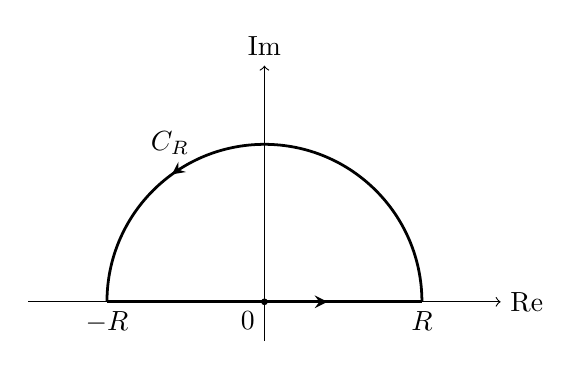
\begin{tikzpicture}
		% Define arrow style for middle placement
		\tikzset{->-/.style={decoration={markings, mark=at position 0.7 with {\arrow{stealth}}}, postaction={decorate}, line width=1.0pt}}
		
		% Draw the x and y axes
		\draw[->] (-3,0) -- (3,0) node[right] {\( \operatorname{Re} \)};
		\draw[->] (0,-0.5) -- (0,3) node[above] {\( \operatorname{Im} \)};
		
		% Draw the horizontal line with an arrow in the middle
		\draw[thick,->-] (-2,0) -- (2,0);
		
		% Draw the semicircle path in counterclockwise direction with an arrow in the middle
		\draw[thick,->-] (2,0) arc[start angle=0, end angle=180, radius=2];
		
		% Add labels
		\node at (2,0) [below] {\( R \)};
		\node at (-2,0) [below] {\( -R \)};
		\node at (-1.2,1.75) [above] {\( C_R \)};
		
		% Optional: add a center point if needed
		\filldraw[black] (0,0) circle (1pt) node[below left] {\( 0 \)};
	\end{tikzpicture}
\end{center}
By the residue theorem,
\begin{align}
	\int_{-R}^R\frac{P(z)}{Q(z)}\,dz+\int_{C_R}\frac{P(z)}{Q(z)}\,dz=2\pi i\sum_{j=1}^n\res\left(\frac{P}{Q},z_j\right),\label{resration}
\end{align}
where $z_1,\cdots,z_n$ are roots of $Q(z)$ in the semicircle region enclosed by $[-R,R]$ and $C_R$. The integrand decays like $R^{-2}$, i.e. there exists a constant $C>0$ such that
\begin{align*}
	\sup_{z\in\bbC:\vert z\vert=R}\left\vert\frac{P(z)}{Q(z)}\right\vert\leq\frac{C}{R^2},
\end{align*}
for sufficiently large $R>0$, we have
\begin{align*}
	\left\vert\int_{C_R}\frac{P(z)}{Q(z)}\,dz\right\vert\leq\frac{\pi C}{R}\to 0,\quad as\ R\to\infty.
\end{align*}
Therefore, letting $R\to\infty$ in (\ref{resration}), we have
\begin{align*}
	\int_{-\infty}^\infty\frac{P(z)}{Q(z)}\,dz=2\pi i\sum_{j=1}^n\res\left(\frac{P}{Q},z_j\right),
\end{align*}
where $z_1,\cdots,z_n$ are roots of $Q(z)$ lying in the upper half plane.
\end{proof}
\paragraph{Remark.} The poles of $\frac{P(z)}{Q(z)}$ are all roots of the polynomial $Q(z)$. If $z_j$ is a root of $Q(z)$ of multiplicity $1$, namely $z_j$ is a simple pole, one can calculate the residue of $\frac{P(z)}{Q(z)}$ by
\begin{align*}
	\res\left(\frac{P}{Q},z_j\right)=P(z_j)\frac{z-z_j}{Q(z)}\bigg|_{z=z_j}.
\end{align*}

\begin{example}[Oscillatory integral]
Let $P$ and $Q$ be two polynomials of single variable. Assume $Q(x)\neq 0$ on $\bbR$, and $\deg(Q)\geq\deg(P)+2$. We want to evaluate the integrals
\begin{align}\label{oscilint}
	\int_{-\infty}^\infty \frac{P(x)}{Q(x)}\sin(x)\,dx\quad and\quad \int_{-\infty}^\infty \frac{P(x)}{Q(x)}\cos(x)\,dx.
\end{align}
\end{example}
\begin{proof}[Solution]
We consider the integral
\begin{align*}
	\int_{-\infty}^\infty \frac{P(x)}{Q(x)}e^{i x}\,dx.
\end{align*}
We continue to use the integral path in Example \ref{rationalint}. By the residue theorem,
\begin{align*}
	\int_{-R}^R\frac{P(x)}{Q(x)}e^{i x}\,dx+\int_{C_R}\frac{P(x)}{Q(x)}e^{i x}\,dx=2\pi i\sum_{j=1}^n\res\left(\frac{P(z)}{Q(z)}e^{i z},z_j\right).
\end{align*}
where $z_1,\cdots,z_n$ are roots of $Q(z)$ lying in the semicircle region enclosed by $[-R,R]$ and $C_R$. According to the M-L estimate, since $\re(i z)\leq 0$ on $C_R$, we have $\vert e^{i z}\vert\leq 1$. Then there exists a constant $C>0$ such that
\begin{align*}
	\sup_{z\in C_R}\left\vert\frac{P(z)}{Q(z)}e^{i z}\right\vert\leq\frac{C}{R^2},
\end{align*}
for sufficiently large $R>0$, we have
\begin{align*}
	\left\vert\int_{C_R}\frac{P(z)}{Q(z)}e^{i z}\,dz\right\vert\leq\frac{\pi C}{R}\to 0,\quad as\ R\to\infty.
\end{align*}
Therefore, letting $R\to\infty$ in (\ref{resration}), we have
\begin{align*}
	\int_{-\infty}^\infty\frac{P(z)}{Q(z)}e^{i z}\,dz=2\pi i\sum_{j=1}^n\res\left(\frac{P(z)}{Q(z)}e^{i z},z_j\right),
\end{align*}
where $z_1,\cdots,z_n$ are roots of $Q(z)$ lying in the upper half plane. The value of the two integrals in (\ref{oscilint}) follows from the real and imaginary part of the last display.
\end{proof}
\begin{lemma}[Jordan's lemma]\label{jordanlemma}
Let $P(z)$ and $Q(z)$ be polynomials with $\deg(Q)\geq\deg(P)+1$. If $m>0$,
\begin{align*}
	\lim_{R\to\infty}\int_{C_R}\frac{P(z)}{Q(z)}e^{i mz}\,dz=0,
\end{align*}
where $C_R$ is the upper semicircle $\{Re^{i\theta},0\leq\theta\leq\pi\}$ from $\theta=0$ to $\pi$. The same conclusion also holds when $m<0$ and $C_R$ is the lower semicircle $\{Re^{i\theta},\pi\leq\theta\leq2\pi\}$ from $\theta=\pi$ to $2\pi$.
\end{lemma}
\begin{proof}
We only need to show the case $\deg(Q)=\deg(P)+1$, otherwise one can apply M-L estimate. Assume $m>0$. Then for $\vert z\vert\gg 1$ great enough, we have
\begin{align*}
\left\vert\frac{P(z)}{Q(z)}\right\vert\leq\frac{K}{\vert z\vert},
\end{align*}
where $K>0$ is an appropriate constant. We parameterize $C_R$ by $\{Re^{i\theta},0\leq\theta\leq\pi\}$. Then
\begin{align*}
	\left\vert\int_{C_R}\frac{P(z)}{Q(z)}e^{i mz}\,dz\right\vert=\left\vert\int_0^\pi\frac{P(Re^{i\theta})}{Q(Re^{i\theta})}e^{i mRe^{i\theta}}\,i Re^{i\theta}\,d\theta\right\vert\leq K\int_0^\pi e^{-mR\sin\theta}\,d\theta.
\end{align*}
Since $\sin\theta\geq\frac{2\theta}{\pi}$ for $0\leq\theta\leq\frac{\pi}{2}$, we have
\begin{align*}
	K\int_0^\pi e^{-mR\sin\theta}\,d\theta\leq 2K\int_0^{\pi/2}e^{-mR\sin\theta}\,d\theta\leq 2K\int_0^{\pi/2}e^{-\frac{2\theta}{\pi}mR}\,d\theta=\frac{\pi K}{mR}\left(1-e^{-mR}\right).
\end{align*}
This bound converges to $0$ as $R\to\infty$. The case $m<0$ is similar.
\end{proof}
\begin{example}[Principal value integral]
We consider the integral
\begin{align*}
	\int_{-\infty}^\infty\frac{\sin(x)}{x}\,dx.
\end{align*}
The integrand decays like $x^{-1}$, and the integral does not converge absolutely. Nevertheless, we can still evaluate the principal value of this integral, which is defined as
\begin{align*}
	\int_{-\infty}^{\infty}\frac{\sin(x)}{x}\,dx=\lim_{R\to\infty}\int_{-R}^R\frac{\sin(x)}{x}\,dx
\end{align*}
\end{example}
\begin{proof}[Solution]
We consider the function $f(z)=\frac{e^{i z}}{z}$ and the integral path consisting of four parts: the upper semicircle $C_R=\{Re^{i\theta},0\leq\theta\leq\pi\}$ from $\theta=0$ to $\pi$, the line segment $[-R,-r]$, the lower semicircle $C_r=\{re^{i\theta},\pi\leq\theta\leq 2\pi\}$ from $\theta=\pi$ to $2\pi$, and the line segment $[r,R]$.
\begin{center}
	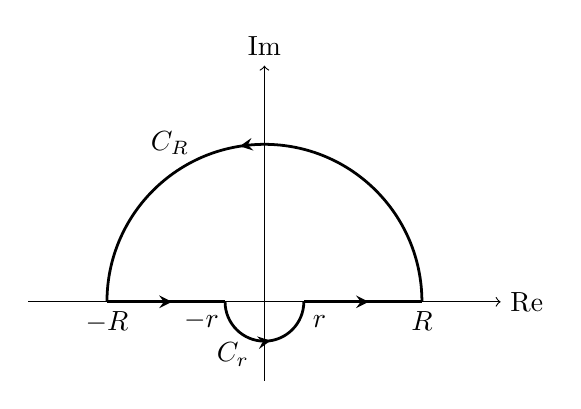
\begin{tikzpicture}
		% Define arrow style for middle placement
		\tikzset{->-/.style={decoration={markings, mark=at position 0.55 with {\arrow{stealth}}}, postaction={decorate}, line width=1.0pt}}
		
		% Draw the x and y axes
		\draw[->] (-3,0) -- (3,0) node[right] {\( \operatorname{Re} \)};
		\draw[->] (0,-1) -- (0,3) node[above] {\( \operatorname{Im} \)};
		
		% Draw the horizontal line with an arrow in the middle
		\draw[thick,->-] (-2,0) -- (-0.5,0);
		\draw[thick,->-] (0.5,0) -- (2,0);
		
		% Draw the semicircle path in counterclockwise direction with an arrow in the middle
		\draw[thick,->-] (2,0) arc[start angle=0, end angle=180, radius=2];
		\draw[thick,->-] (-0.5,0) arc[start angle=180, end angle=360, radius=0.5];
		
		% Add labels
		\node at (2,0) [below] {\( R \)};
		\node at (-2,0) [below] {\( -R \)};
		\node at (0.7,-0.05) [below] {\( r \)};
		\node at (-0.8,0) [below] {\( -r \)};
		\node at (-1.2,1.75) [above] {\( C_R \)};
		\node at (-0.4,-0.4) [below] {\( C_r \)};
	\end{tikzpicture}
\end{center}
By the residue theorem,
\begin{align*}
	\int_{-R}^{-r}f(z)\,dz+\int_{C_r}f(z)\,dz+\int_r^Rf(z)\,dz+\int_{C_R}f(z)\,dz=2\pi i\res\left(f,0\right)=2\pi i.
\end{align*}
According to Lemma \ref{jordanlemma}, the integral on $C_R$ converges to $0$ as $R\to 0$. For the integral on $C_r$, note that
\begin{align*}
\int_{C_r}\frac{e^{iz}}{z}\,dz&=\int_{C_r}\frac{1}{z}\,dz+\int_{C_r}\frac{e^{iz}-1}{z}\,dz\\
&=\int_\pi^{2\pi}\frac{1}{re^{i\theta}}ire^{i\theta}\,d\theta+\int_{C_r}\frac{e^{iz}-1}{z}\,dz=\pi i+\int_{C_r}\frac{e^{iz}-1}{z}\,dz.
\end{align*}
The function $z\mapsto\frac{e^{iz}-1}{z}$ is holomorphic, hence is bounded near $z=0$. Then the integral $\int_{C_r}\frac{e^{iz}-1}{z}\,dz$ converges to $0$ as $r\to 0$. Therefore
\begin{align*}
	P.V.\int_{-\infty}^{\infty}\frac{e^{ix}}{x}\,dx=\lim_{r\to 0,R\to\infty}\left(\int_{-R}^{-r}f(z)\,dz+\int_r^Rf(z)\,dz\right)=\pi\i
\end{align*}
Taking the imaginary part, we have $\int_{-\infty}^\infty\frac{\sin(x)}{x}=\pi$.
\end{proof}

\begin{example}[Trigonometric rational functions on the unit circle] Let $P$ and $Q$ be two polynomials of two variables, and define $R=\frac{P}{Q}$. We want to evaluate the integral
\begin{align*}
	\int_0^{2\pi}R(\cos\theta,\sin\theta)\,d\theta.
\end{align*}
\end{example}
\begin{proof}[Solution]
By changing the variable $z=e^{i\theta}$,
\begin{align*}
\int_0^{2\pi} f(e^{i\theta})\,d\theta=\int_0^{2\pi} \frac{f(e^{i\theta})}{ie^{i\theta}}\,de^{i\theta}=\int_{\vert z\vert=1}\frac{f(z)}{iz}\,dz.
\end{align*}
Since $\cos\theta=\frac{1}{2}\left(z+\frac{1}{z}\right)$, and $\sin\theta=\frac{1}{2\i}\left(z-\frac{1}{z}\right)$, we have
\begin{align*}
	\int_0^{2\pi}R(\cos\theta,\sin\theta)\,d\theta=\int_{\vert z\vert=1}\frac{1}{iz}R\left(\frac{z^2+1}{2z},\frac{z^2-1}{2iz}\right)\,dz.
\end{align*}
The integrand is also a rational function of $z$:
\begin{align*}
	g(z)=\frac{1}{iz}R\left(\frac{z^2+1}{2z},\frac{z^2-1}{2iz}\right)
\end{align*}
Then we can compute the integral by
\begin{align*}
	\int_0^{2\pi}R(\cos\theta,\sin\theta)\,d\theta=2\pi i\sum_{j=1}^n\res(g,z_j),
\end{align*}
where $z_1,z_2,\cdots,z_n$ are poles of $g$ inside the unit disk $\vert z\vert<1$. 
\end{proof}

\begin{example}[Sector contours]
We want to evaluate the following integral:
\begin{align*}
	\int_0^\infty\frac{dx}{1+x^n},\quad n=2,3,\cdots.
\end{align*}
\end{example}
\begin{proof}[Solution]
We consider the integral path round a sector of radius $r$ and angle $\frac{2\pi}{n}$, which consists of segment $[0,R]$, the arc $C_R=\left\{Re^{i\theta},0\leq\theta\leq\frac{2\pi}{n}\right\}$ and the segment $\bigl[Re^{\frac{2\pi i}{n}},0\bigr]$. The function $f(z)=\frac{1}{1+z^n}$ has a simple pole at $e^{\frac{i\pi}{n}}$ inside the sector when $R>1$.
\begin{center}
	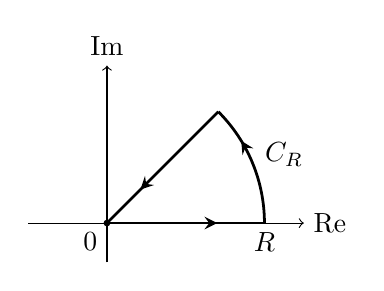
\begin{tikzpicture}
		% Define arrow style for middle placement
		\tikzset{->-/.style={decoration={markings, mark=at position 0.7 with {\arrow{stealth}}}, postaction={decorate}, line width=1.0pt}}
		
		% Draw the x and y axes
		\draw[->] (-1,0) -- (2.5,0) node[right] {\( \operatorname{Re} \)};
		\draw[->] (0,-0.5) -- (0,2) node[above] {\( \operatorname{Im} \)};
		
		% Draw the horizontal line with an arrow in the middle
		\draw[thick,->-] (0,0) -- (2,0);
		\draw[thick,->-] (1.414,1.414) -- (0,0);
		
		% Draw the semicircle path in counterclockwise direction with an arrow in the middle
		\draw[thick,->-] (2,0) arc[start angle=0, end angle=45, radius=2];
		
		% Add labels
		\node at (2,0) [below] {\( R \)};
		\node at (2.25,0.6) [above] {\( C_R \)};
		
		% Optional: add a center point if needed
		\filldraw[black] (0,0) circle (1pt) node[below left] {\( 0 \)};
	\end{tikzpicture}
\end{center}
By the residue theorem,
\begin{align*}
	\int_0^R\frac{dz}{1+z^n}+\int_{C_R}\frac{dz}{1+z^n}+\int_{Re^{\frac{2\pi i}{n}}}^0\frac{dz}{1+z^n}=2\pi i\res\left(\frac{1}{1+z^n},e^{\frac{i\pi}{n}}\right).
\end{align*}
The integral on $C_R$ converges to $0$ by M-L estimate. The integral on the segment $\bigl[Re^{\frac{2\pi i}{n}},0\bigr]$ is
\begin{align*}
	\int_R^0\frac{e^{\frac{2\pi i}{n}}dx}{1+\bigl(xe^{\frac{2\pi i}{n}}\bigr)^n}=-e^{\frac{2\pi i}{n}}\int_0^R\frac{dx}{1+x^n}.
\end{align*}
Letting $R\to\infty$, we have
\begin{align*}
	\left(1-e^{\frac{2\pi i}{n}}\right)\int_0^\infty\frac{dx}{1+x^n}=2\pi i\res\left(\frac{1}{1+z^n},e^{\frac{i\pi}{n}}\right).
\end{align*}
It remains to calculate the residue:
\begin{align*}
	\res\left(\frac{1}{1+z^n},e^{\frac{i\pi}{n}}\right)=\frac{1}{nz^{n-1}}\bigg|_{z=e^{\frac{i\pi}{n}}}=-\frac{1}{n}e^{\frac{i\pi}{n}}.
\end{align*}
Therefore,
\begin{align*}
	\int_0^\pi\frac{dx}{1+x^n}=\frac{2\pi i}{n\bigl(e^{\frac{2\pi i}{n}}-1\bigr)}e^{\frac{\pi\i}{n}}=\frac{2\pi i}{n\bigl(e^{\frac{\pi\i}{n}}-e^{-\frac{\pi\i}{n}}\bigr)}=\frac{\pi}{n\sin\left(\frac{\pi}{n}\right)}.
\end{align*}
This formula holds for all integers $n$ greater than $1$.
\end{proof}

\newpage
\section{Miscellaneous}
\subsection{Analytic Continuation}
We first introduce the uniqueness theorem for analytic functions.
\begin{theorem}[Uniqueness theorem for analytic functions]\label{analuniq}
Let $f$ be an analytic function in an open connected domain such that $f(z_n)=0$ for a sequence $(z_n)_{n=1}^\infty$ of distinct points with $z_n\to z_0\in U$. Then $f\equiv 0$ in $U$.
\end{theorem}
\begin{proof}
Since $f$ is analytic at $z_0$, it has a power series representation around $z_0$. By the uniqueness theorem for power series [Theorem \ref{pwsruniq}], $f\equiv 0$ throughout some open disc containing $z_0$. To show that $f\equiv 0$ in $U$, we partition $U$ into two sets:
\begin{align*}
	A=\left\{z\in U:z\ is\ a\ limit\ of\ zeros\ of\ f\right\},\quad B=U\backslash A.
\end{align*}
For each $z\in A$, since it is a limit of zeros of $f$, we know that $f\equiv 0$ in some open disc containing $z$, and $z\in\mathring{A}$. Hence $A$ is an open set. On the other hand for each $z\in B$, we have $f(\omega)\neq 0$ in a punctured disc $0<\vert\omega-z\vert<\delta$, and $z\in\mathring{B}$. Hence $B$ is also an open set. By connectedness of $U$, either $A$ or $B$ is empty. Since $z_0\in A$, $B$ is empty, and every $z\in U$ is a limit of zeroes of $f$. By continuity, $f\equiv 0$ throughout $U$.
\end{proof}
\begin{corollary}
Let $U$ be an open connected domain $U$. If two analytic functions $f$ and $g$ in $U$ agree at a set of points with a limit point in $U$, then $f\equiv g$ through $U$.
\end{corollary}
\begin{proof}
Consider the function $f-g$ and apply Theorem \ref{analuniq}.
\end{proof}
Suppose we are given a function $f$ which is analytic in an open domain $U$. We say that $f$ can be \textit{continued analytically} to an open domain $U_1$ that intersects $U$ if there exists a function $g$, analytic in $U$ and such that $g = f$ throughout $U\cap U_1$. By the uniqueness theorem, any such continuation of $f$ is uniquely determined. 
\begin{definition}[Regularity]
Let $f$ be an analytic function in an open disc $D$. If $z_0\in\partial D$ and and $f$ can be continued analytically to an open neighborhood $U$ of $z_0$, then $f$ is said to be \textit{regular at $z_0$}. Otherwise, $f$ is said to have a \textit{singularity} at $z_0$. 
\end{definition}
We first discuss the analytical continuation of power series.
\begin{theorem}\label{analcontsing}
If the power series $\sum_{n=0}^\infty c_nz^n$ has a positive radius of convergence $R<\infty$, the function $f(z)=\sum_{n=0}^\infty c_nz^n$ has at least one singularity on the circle $\vert z\vert=R$.
\end{theorem}
\begin{proof}
Argue by contradiction. If $f$ has no singularities on $\vert z\vert=R$, we can choose an open disc $B(z,\epsilon_z)$ to which $f$ can be continued analytically for each $\vert z\vert=R$. By taking the union of $B(0,R)$ and these discs centered on $\vert z\vert=R$, we obtain an open connected domain $U$ to which $f$ can be continued analytically. 

We consider the function $d(z,U^c)=\inf_{y\in U^c}\vert y-z\vert$, which is continuous on $z\in\ol{B(0,R)}$. By compactness, there exists $\epsilon>0$ such that $d(z,U^c)>\epsilon$ for all $z\in\ol{B(0,R)}$. Hence the disc $B(0,R+\epsilon)$ lies in $U$. Using the uniqueness theorem [Theorem \ref{pwsruniq}], the continuation $g$ of $f$ on $B(0,R+\epsilon)$ has the same power series representation $\sum_{n=0}c_nz^n$, which is convergent for all $\vert z\vert <R+\epsilon$. But $\sum_{n=0}^\infty c_nz^n$ has radius of convergence $R$, which leads to a contradiction.
\end{proof}

\begin{theorem}
If the power series $\sum_{n=0}^\infty c_nz^n$ has a positive radius of convergence $R<\infty$ and $c_n\geq 0$ for all $n\in\bbN_0$, the function $f(z)=\sum_{n=0}^\infty c_nz^n$ has a singularity at $z=R$.
\end{theorem}
\begin{proof}
By Theorem \ref{analcontsing}, $f$ has singularity at some $Re^{i\theta}$. Consider the power series for $f$ about a point $\rho e^{i\theta}$, with $0<\rho<R$:
\begin{align*}
	f(z)=\sum_{n=0}^\infty a_n(z-\rho e^{i\theta})^n=\sum_{n=0}^\infty\frac{f^{(n)}(\rho e^{i\theta})}{n!}(z-\rho e^{i\theta})^n.
\end{align*}
The radius of convergence of this series is $R-\rho$. Furthermore, for any nonnegative integer $k$,
\begin{align*}
	f^{(k)}(\rho e^{i\theta})=\sum_{n=k}^\infty n(n-1)\cdots(n-k+1)c_n(\rho e^{i\theta})^{n-k}.
\end{align*}
Since $c_n\geq 0$, we have $\vert f^{(k)}(\rho e^{i\theta})\vert\leq f^{(k)}(\rho)$. By Theorem \ref{powercvg}, the power series expansion of $f$ at $\rho$,
\begin{align*}
	\sum_{n=0}^\infty\frac{f^{(n)}(\rho)}{n!}(z-\rho)^n,
\end{align*}
has radius of convergence $R-\rho$. On the other hand, if $f$ were regular at $z = R$, the above power series would converge in a disc of radius greater than $R-\rho$. Therefore $f$ is singular at $z=R$.
\end{proof}
\begin{definition}[Natural boundary]
If $f(z)=\sum_{n=0}^\infty c_nz^n$ has a singularity at every point on its circle of convergence, then that circle is called a \textit{natural boundary of $f$}.
\end{definition}

The following criterion is useful for determining the natural boundary of power series.
\begin{theorem}[Ostrowski-Hadamard gap theorem]
Let $f(z)=\sum_{k=0}^\infty c_kz^{n_k}$ be a power series with a positive radius of convergence $R<\infty$. If $$\liminf_{k\to\infty}\frac{n_{k+1}}{n_k}>1,$$ the circle of convergence of the power series is a natural boundary for $f$. 
\end{theorem}
\begin{proof}
Since the result is independent of $c_k$, we may assume without loss of generality that the radius of convergence is $1$. Also, by neglecting finitely many terms if necessary, we may assume that for some $\delta>0$ and for all $k$, it holds $n_{k+1}/n_k > 1+\delta$. Finally, it suffices
to show that $f$ is singular at the point $z = 1$. For the same result, applied to the series $\sum_{k=0}^\infty c_k(ze^{-i\theta})^{n_k}$, shows that $f$ is singular at any point $z=e^{i\theta}$.

Choose an integer $m>\delta^{-1}$ and consider the power
series $g(\omega)$ obtained by setting $z=\frac{\omega^m+\omega^{m+1}}{2}$
and in $f$ and expanding the terms:
\begin{align*}
	g(\omega)&=f\left(\frac{\omega^m+\omega^{m+1}}{2}\right)=\frac{c_0}{2^{n_0}}\omega^{mn_0}+\frac{c_0n_0}{2^{n_0}}\omega^{mn_0+1}+\frac{c_0n_0(n_0+1)}{2\cdot 2^{n_0}}\omega^{mn_0+2}+\cdots+\frac{c_0}{2^{n_0}}\omega^{mn_0+n_0}\\
	&\quad +\frac{c_1}{2^{n_1}}\omega^{mn_1}+\frac{c_1n_1}{2^{n_1}}\omega^{mn_1+1}+\frac{c_1n_1(n_1+1)}{2\cdot 2^{n_1}}\omega^{mn_1+2}+\cdots+\frac{c_1}{2^{n_1}}\omega^{mn_1+n_1}+\cdots.
\end{align*}
Note that in this expression no two terms involve the same power of $\omega$, since
\begin{align*}
	mn_{k+1}>mn_k+n_k\quad\mathrm{whenever}\quad \frac{n_{k+1}}{n_k}>1+\frac{1}{m}.
\end{align*}
When $\vert\omega\vert<1$, we have $z=\frac{\omega^m+\omega^{m+1}}{2}<1$, hence $g(\omega)=f(z)$ is absolutely convergent. On the other hand, if we take $\omega>1$, we have $z=\frac{\omega^m+\omega^{m+1}}{2}>1$, and $g(\omega)$ diverges. Hence the power series $g(\omega)$ has radius of convergence $1$. By Theorem \ref{analcontsing}, $g$ must have a singularity at some $\omega_0$ with $\vert\omega_0\vert=1$. If $\omega_0\neq 1$, 
\begin{align*}
	\left\vert\frac{\omega^m+\omega^{m+1}}{2}\right\vert=\vert\omega\vert^m\left\vert\frac{1+\omega}{2}\right\vert<1.
\end{align*}
Since $f(z)$ is analytic in $\vert z\vert<1$, $g$ is regular at $\omega_0$. Thus $g$ must have a singularity at $\omega_0=1$, and since $$g(\omega)=f\left(\frac{\omega^m+\omega^{m+1}}{2}\right),$$ $f(z)$ must have a singularity at $z=1$.
\end{proof}

\subsection{Holomorphic Functions Defined by Integrals}
\begin{theorem}[Holomorphy of definite integrals]
Let $F(z,t)$ be a continuous function of $z\in U\subset\bbC$ and $t\in[a,b]$, where $U$ is an open domain in $\bbC$. If $F$ is holomorphic in $z$ for each fixed $t\in[a,b]$, then
\begin{align*}
	f(z)=\int_a^b F(z,t)\,dt
\end{align*}
is holomorphic in $U$, and the complex derivative is
\begin{align*}
	f^\prime(z)=\int_a^b\frac{\partial F}{\partial z}(z,t)\,dt.
\end{align*}
\end{theorem}
\begin{proof}
We first claim that the first and second partial derivatives $F_z$ and $F_{zz}$ are continuous as functions of two variables. By Cauchy's integral theorem,
\begin{align*}
	F(z,t)=\frac{1}{2\pi i}\int_C\frac{F(\omega,t)}{\omega-z}\,d\omega,\quad F_z(z,t)=\frac{1}{2\pi i}\int_C\frac{F(\omega,t)}{(\omega-z)^2}\,d\omega,\quad F_{zz}(z,t)=\frac{1}{\pi i}\int_C\frac{F(\omega,t)}{(\omega-z)^3}\,d\omega,
\end{align*}
where $C$ is any contour in $U$ enclosing $z$. Given $z_0\in U$, we let $C$ be the boundary of a closed disc $\ol{B(z_0,r)}$ contained in $U$. Since $F$ is uniformly continuous on the compact set $\ol{B(z_0,r)}\times[a,b]$, and on $C\times [a,b]$, we let $M=\max_{\omega\in C,t\in[a,b]}F(\omega,t)$. Then for all $z\in B(z_0,\epsilon)$ with $\epsilon<r$,
\begin{align*}
\left\vert\int_C\frac{F(\omega,t)}{(\omega-z)^2}\,d\omega-\int_C\frac{F(\omega,t)}{(\omega-z_0)^2}\,d\omega\right\vert&\leq 2\pi rM\max_{\omega\in C}\left\vert\frac{1}{(\omega-z)^2}-\frac{1}{(\omega-z_0)^2}\right\vert\leq\frac{4\pi r^2M\epsilon}{(r-\epsilon)^4},
\end{align*}
and by uniform continuity of $F$ on $C\times[a,b]$,
\begin{align*}
	\lim_{t^\prime\to t}\left\vert\int_C\frac{F(\omega,t)}{(\omega-z_0)^2}\,d\omega-\int_C\frac{F(\omega,t^\prime)}{(\omega-z_0)^2}\,d\omega\right\vert=0.
\end{align*}
Hence $F_z$ is continuous. The continuity of $F_{zz}$ follows in a similar approach. We then consider the expansion
\begin{align*}
	F(z,t)=F(z_0,t)+F_z(z_0,t)(z-z_0)+R(z,t),\quad z\in B(z_0,r),
\end{align*}
where the remainder $R(z,t)$ satisfies a uniform estimate of the form
\begin{align*}
	\left\vert R(z,t)\right\vert\leq A\vert z-z_0\vert^2, \quad A=\max_{z\in \ol{B(z_0,r)},\,t\in[a,b]}\vert F_{zz}(z,t)\vert.
\end{align*}
For all $z\in B(z_0,r)$,
\begin{align*}
	\left\vert\int_a^b\left(\frac{F(z,t)-F(z_0,t)}{z-z_0}- F_z(z_0,t)\right)dt\right\vert\leq\int_a^b A\vert z-z_0\vert\,dt=A(b-a)\vert z-z_0\vert.
\end{align*}
Hence $\int_a^b F(z,t)\,dt$ is holomorphic in $z$, and the derivative is $\int_a^b F_z(z,t)\,dt$. Thus we complete the proof.
\end{proof}
\paragraph{Remark.} The same conclusion does not necessarily hold if we replace the compact interval $[a,b]$ by a non-compact one. For example,
\begin{align*}
	f(z)=\int_{-\infty}^\infty\frac{e^{itz}}{1+t^2}\,dt
\end{align*}
is not holomorphic in $z$. In fact, the integral does not converges when $z\notin \bbR$.
\begin{theorem}[Holomorphy of improper integrals]\label{compactconvgint}
Let $F(z,t)$ be a continuous function of $z\in U\subset\bbC$ and $t\in(0,\infty)$, where $U$ is an open domain in $\bbC$. Assume that $F$ is holomorphic in $z$ for each fixed $t\in(0,\infty)$, and the improper integral
\begin{align*}
	f(z)=\int_0^\infty F(z,t)\,dt
\end{align*}
is absolutely convergent for all $z\in U$. Furthermore, assume that for all compact $K\subset U$,
\begin{align*}
	\lim_{a\to 0^+,\,b\to\infty}\sup_{z\in K}\left\vert\int_a^b F(t,z)\,dt-f(z)\,dt\right\vert=0.
\end{align*}
In other words, the improper integral converges uniformly in $z$ on any compact subset of $U$. Then $f(z)$ is holomorphic in $U$, and
\begin{align}
	f^\prime(z)=\int_0^\infty\frac{\partial F}{\partial z}(z,t)\,dt.\label{improperintderiv}
\end{align}
\end{theorem}
\begin{proof}
The previous theorem implies that $$f_n(z)=\int_{\frac{1}{n}}^n F(z,t)\,dt,\quad n=1,2,\cdots$$ is a sequence of holomorphic functions in $U$. By our assumption, $f_n\to f$ pointwise and compactly. Using Theorem \ref{compactholoconvg}, we know that $f(z)$ is also holomorphic in $U$. By Cauchy's integral formula and Theorem [\ref{unifconvergence}],
\begin{align*}
	f^\prime(z)=\frac{1}{2\pi i}\int_C\frac{f(z)}{(\omega-z)^2}\,d\omega=\lim_{n\to\infty}\frac{1}{2\pi i}\int_C\frac{f_n(z)}{(\omega-z)^2}\,d\omega=\lim_{n\to\infty} f_n^\prime(z),
\end{align*}
where we choose $C$ to be a circle around $z$ and contained in $U$. Then the derivative formula (\ref{improperintderiv}) follows.
\end{proof}

\subsection{The Gamma Function}
\paragraph{Gamma function in the right half-plane.} We consider the improper integral
\begin{align*}
	\Gamma(s)=\int_0^\infty t^{s-1}e^{-t}\,dt,
\end{align*}
where $s\in\bbC$, and the power $t^{s-1}$ is defined by $e^{(s-1)\log t}$. The integral converges absolutely when $\re(s)>0$. Furthermore, we fix some compact set $K\subset\{z:\re(z)>0\}$ with $0<\kappa<\re(s)<\sigma$ for all $s\in K$. When we take the integral near infinity, we obtain the following uniform estimate for $s\in K$: 
\begin{align*}
	\left\vert\int_b^\infty t^{s-1}e^{-t}\,dt\right\vert&\leq\int_b^\infty t^{\re(s)-1}e^{-t}\,dt\leq\int_b^\infty e^{-\frac{t}{2}}\,dt\times\sup_{t\geq b}e^{-\frac{t}{2}}t^{\re(s)-1}\leq 2e^{-\frac{b}{2}}\sup_{t\geq b}e^{-\frac{t}{2}}t^{\sigma-1}.
\end{align*}
Clearly, this estimate converges to $0$ as $b\to\infty$. On the other hand, we also the following uniform estimate for $s\in K$ when we take the integral near $0$:
\begin{align*}
	\left\vert\int_0^a t^{s-1}e^{-t}\,dt\right\vert&\leq\int_0^a t^{\re(s)-1}e^{-t}\,dt\leq\int_0^a t^{\kappa-1}\,dt\leq\frac{a^{\kappa}}{\kappa}.
\end{align*}
Again this estimate converges to $0$ when $a\to 0$. Hence we verified the compact convergence condition in Theorem \ref{compactconvgint}. To conclude, the Gamma function $\Gamma(s)$ is holomorphic in the right-half plane $\re(s)>0$. Next, we are going to extend this function to the whole plane.

\paragraph{Meromorphic continuation of $\Gamma$ to $\bbC$.} Use the integration by parts formula, we see that
\begin{align*}
\Gamma(s+1)=\int_0^\infty t^se^{-t}\,dt=t^se^t\big|_{t=0}^{t=\infty}+s\int_0^\infty e^{-t}t^{s-1}\,dt=s\Gamma(s),\quad\re(s)>0.
\end{align*}
This identity allows us to define an extension of $\Gamma$ to the half-plane $\re(s)>-1,\ s\neq 0$:
\begin{align*}
\Gamma(s)=\frac{\Gamma(s+1)}{s},\quad\re(s)>-1,\ s\neq 0.
\end{align*}
Clearly, the extended $\Gamma$ is holomorphic in both $\re(s)>0$ and $-1<\re(s)<0$, and continuous on the nonzero imaginary axis $\{iy:y\neq 0\}$. By Theorem \ref{segmentext}, the extended $\Gamma$ is holomorphic throughout $\re(s)>1,\ s\neq 0$. Furthermore, we have $\Gamma(s)\sim\frac{1}{s}$ near $s=0$, since
\begin{align*}
	\lim_{s\to 0}s\Gamma(s)=\lim_{s\to 0}\Gamma(s+1)=0.
\end{align*}
Hence $\Gamma$ has a simple pole at $s=0$ with residue $1$. We repeat the same manner and define
\begin{align*}
	\Gamma(s)&=\frac{\Gamma(s+2)}{s(s+1)},\quad\re(s)>-2,\ s\neq 0,-1,\\
	\Gamma(s)&=\frac{\Gamma(s+3)}{s(s+1)(s+2)},\quad\re(s)>-3,\ s\neq 0,-1,-2,\\
	\cdots,\\
	\Gamma(s)&=\frac{\Gamma(s+k+1)}{s(s+1)\cdots(s+k)},\quad\re(s)>-k-1,\ s\neq 0,-1,\cdots,-k.
\end{align*}
Then we obtain an extended $\Gamma$ that is meromorphic on $\bbC$ with poles only at nonpositive integers. Moreover, near $s=-k$, where $k\in\bbN_0$,
\begin{align*}
	\lim_{s\to -k}(s+k)\Gamma(s)=\lim_{s\to -k}\frac{\Gamma(s+k+1)}{s(s+1)\cdots(s+k-1)}=\frac{(-1)^k}{k!}.
\end{align*}
Hence
\begin{align*}
	\res(\Gamma,-k)=\frac{(-1)^k}{k!},\quad k=0,-1,-2,\cdots.
\end{align*}
Thus we get an meromorphic continuation of $\Gamma$ on the entire complex plane.
\paragraph{Euler-Mascheroni constant.} We consider the sequence $t_n=1+\frac{1}{2}+\cdots+\frac{1}{n-1}-\log n$. One can easily verify that $(t_n)$ is a bounded monotone increasing sequence:
\begin{align*}
	t_n&=1+\frac{1}{2}+\cdots+\frac{1}{n-1}-\log n=\sum_{k=1}^{n-1}\left(\frac{1}{k}-\log\frac{k+1}{k}\right)\\
	&\leq\sum_{k=1}^{n-1}\frac{1}{2k^2}\leq\sum_{k=1}^\infty\frac{1}{2k^2}=\frac{\pi^2}{12}.
\end{align*}
Hence the sequence $(t_n)$ is convergent, and its limit $\lim_{n\to\infty}t_n$ equals
\begin{align*}
	\gamma=\lim_{n\to\infty}\left(1+\frac{1}{2}+\cdots+\frac{1}{n}-\log n\right)\approx 0.5772156649.
\end{align*}
This limit is called the \textit{Euler-Mascheroni constant}. This constant is related to the gamma function.

\begin{theorem}[Gauss] The $\Gamma$ function can be written as
	\begin{align}
		\Gamma(s)=\lim_{n\to\infty}\frac{n!\,n^s}{s(s+1)\cdots(s+n)},\quad s\in\bbC,\ s\neq 0,-1,-2,\cdots.\label{gaussgamma}
	\end{align}
\end{theorem}
\begin{proof}
By calculus, we have
$e^{-t/n}-\left(1-\frac{t}{n}\right)\leq\frac{t^2}{2n^2}$. Applying the inequality $a^n-b^n\leq na^{n-1}(a-b)$ for $a>b$ and $n\geq 1$ gives\vspace{-0.1cm}
\begin{align*}
	e^{-t}-\left(1-\frac{t}{n}\right)^n\leq \frac{t^2e^{-(1-\frac{1}{n})t}}{2n}\leq\frac{t^2e^{-t/2}}{2n}\leq\frac{8}{ne^2},\quad n\geq 2.
\end{align*}
Hence $\left(1-\frac{t}{n}\right)^n\to e^{-t}$ uniformly on $(0,\infty)$. We plug-in this limit to the integral definition of $\Gamma$ function and apply integration by parts:
\begin{align*}
	\Gamma(s)&=\int_0^\infty t^{s-1}e^{-t}\,dt=\lim_{n\to\infty}\int_0^n t^{s-1}\left(1-\frac{t}{n}\right)^n\,dt=\lim_{n\to\infty}\frac{1}{n^n}\int_0^n t^{s-1}(n-t)^n\,dt\\
	&=\lim_{n\to\infty}\frac{1}{n^n}\cdot\frac{n}{s}\int_0^n t^s(n-t)^{n-1}\,dt=\cdots=\lim_{n\to\infty}\frac{1}{n^n}\cdot\frac{n(n-1)\cdots 1}{s(s+1)\cdots(s+n-1)}\int_0^n t^{s+n-1}\,dt\\
	&=\lim_{n\to\infty}\frac{n!\,n^s}{s(s+1)\cdots(s+n)},\quad\re(s)>0.
\end{align*}
Furthermore, for $\re(s)>-k-1$, we use the continuation given before to get
\begin{align*}
	\Gamma(s)&=\frac{\Gamma(s+k+1)}{s(s+1)\cdots(s+k)}=\lim_{n\to\infty}\frac{n!\,n^{s+k+1}}{s(s+1)\cdots(s+k)\cdot (s+k+1)\cdots(s+k+n+1)}\\
	&=\lim_{n\to\infty}\frac{n!\,n^s}{s(s+1)\cdots(s+n)}\times\lim_{n\to\infty}\frac{n}{s+n+1}\cdot\frac{n}{s+n+2}\cdots\frac{n}{s+n+k+1}\\
	&=\lim_{n\to\infty}\frac{n!\,n^s}{s(s+1)\cdots(s+n)}.
\end{align*}
Therefore we obtain the alternative definition for $\Gamma$.
\end{proof}

\begin{theorem}[Weierstrass-Hadamard product] For all $s\in\bbC$, the reciprocal of $\Gamma(s)$ is
\begin{align*}
	\frac{1}{\Gamma(s)}=se^{\gamma s}\prod_{n=1}^\infty\left(1+\frac{s}{n}\right)e^{-\frac{s}{n}},
\end{align*}
where $\gamma$ is the Euler-Mascheroni constant.
\end{theorem}
\begin{proof}
If $s\neq 0,-1,-2,\cdots$, we insert the factors $e^{-\frac{s}{n}}$ to the reciprocal of (\ref{gaussgamma}) and obtain
\begin{align*}
	\frac{1}{\Gamma(s)}&=\lim_{n\to\infty}sn^{-s}\left(1+s\right)\left(1+\frac{s}{2}\right)\cdots\left(1+\frac{s}{n}\right)\\
	&=\lim_{n\to\infty}se^{s\left(1+\frac{1}{2}+\cdots+\frac{1}{n}-\log n\right)}\left(1+s\right)e^{-s}\left(1+\frac{s}{2}\right)e^{-\frac{s}{2}}\cdots\left(1+\frac{s}{n}\right)e^{-\frac{s}{n}}\\
	&=se^{\gamma s}\prod_{n=1}^\infty\left(1+\frac{s}{n}\right)e^{-\frac{s}{n}}
\end{align*}
For the case $s\neq 0,-1,-2,\cdots$, we have $1/\Gamma(s)=0$, and the result is clear.
\end{proof}

\begin{theorem}[Euler's Reflection formula]\label{eulerrefl}
For all $s\in\bbC$ with $s\neq\bbZ$,
\begin{align*}
	\Gamma(s)\Gamma(1-s)=\frac{\pi}{\sin(s\pi)}.
\end{align*}
\end{theorem}
\begin{proof}
We consider $0<\re(s)<1$. By definition,
\begin{align*}
\Gamma(s)\Gamma(1-s)&=\int_0^\infty\int_0^\infty u^{s-1}e^{-u}v^{-s}e^{-v}\,du\,dv\overset{v=ut}{=}\int_0^\infty\int_0^\infty t^{-s}e^{-u(t+1)}\,du\,dt=\int_0^\infty\frac{t^{-s}}{1+t}\,dt.
\end{align*}
We then apply contour integral to compute the last integral. For the multi-valued function $z^{-s}$, we use the main branch $(re^{i\theta})^{-s}=r^{-s}(e^{-is\theta})$, where $0\leq\theta<2\pi$. Use the keyhole path shown below.
\begin{center}
	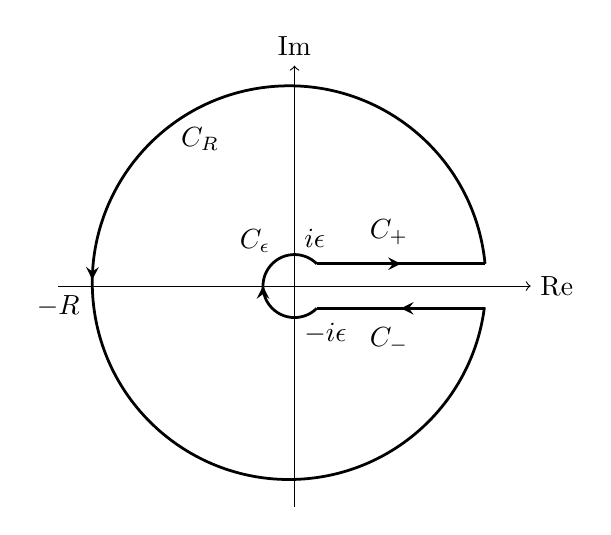
\begin{tikzpicture}
		% Define arrow style for middle placement
		\tikzset{->-/.style={decoration={markings, mark=at position 0.50 with {\arrow{stealth}}}, postaction={decorate}, line width=1.0pt}}
		
		% Draw the x and y axes
		\draw[->] (-3,0) -- (3,0) node[right] {\( \operatorname{Re} \)};
		\draw[->] (0,-2.80) -- (0,2.80) node[above] {\( \operatorname{Im} \)};
		
		% Draw the horizontal line with an arrow in the middle
		\draw[thick,->-] (0.2828,0.2828) -- (2.42,0.2828);
		\draw[thick,->-] (2.42,-0.2828) -- (0.2828,-0.2828);
		
		% Draw the semicircle path in counterclockwise direction with an arrow in the middle
		\draw[thick,->-] (2.42,0.2828) arc[start angle=5.5, end angle=352.8, radius=2.5];
		\draw[thick,->-] (0.2828,-0.2828) arc[start angle=315, end angle=45, radius=0.4];
		
		% Add labels
		\node at (-3,0) [below] {\( -R \)};
		\node at (0,0.6) [right] {\( i\epsilon \)};
		\node at (0,-0.6) [right] {\( -i\epsilon \)};
		\node at (1.2,0.4) [above] {\( C_+ \)};
		\node at (1.2,-0.4) [below] {\( C_- \)};
		\node at (-1.2,1.6) [above] {\( C_R \)};
		\node at (-0.5,0.3) [above] {\( C_\epsilon \)};
	\end{tikzpicture}
\end{center}
By the residue theorem, we have
\begin{align*}
	\int_{\epsilon}^{R}\frac{z^{-s}}{1+z}\,dz+\int_{C_R}\frac{z^{-s}}{1+z}\,dz+\int_{R}^{\epsilon}\frac{z^{-s}e^{-2i\pi s}}{1+z}\,dz+\int_{C_\epsilon}\frac{z^{-s}}{1+z}\,dz=\res\left(\frac{z^{-s}}{1+z},-1\right)=e^{-i\pi s}.
\end{align*}
We use the M-L estimate to eliminate integrals on $C_R$ and $C_\epsilon$. On the outer circle $C_R$,
\begin{align*}
	\left\vert\int_{C_R}\frac{z^{-s}}{1+z}\,dz\right\vert\leq 2\pi R\cdot\frac{R^{-\re(s)}}{R-1}\sim 2\pi R^{-\re(s)}\to 0,\quad\text{as}\ \ R\to\infty.
\end{align*}
On the inner circle $C_\epsilon$,
\begin{align*}
	\left\vert\int_{C_\epsilon}\frac{z^{-s}}{1+z}\,dz\right\vert\leq 2\pi\epsilon\cdot\frac{\epsilon^{-\re(s)}}{1-\epsilon}\sim 2\pi\epsilon^{1-\re(s)}\to 0,\quad\text{as}\ \ \epsilon\to 0^+.
\end{align*}
Letting $\epsilon\to 0^+$ and $R\to\infty$, we have
\begin{align*}
	\int_{0}^{\infty}\frac{z^{-s}}{1+z}\,dz-e^{-2i\pi s}\int_{0}^\infty\frac{z^{-s}}{1+z}\,dz=e^{-i\pi s}.
\end{align*}
Hence
\begin{align*}
	\int_0^\infty\frac{t^{-s}}{1+t}\,dt=\frac{2\pi i}{1-e^{-2i\pi s}}e^{-i\pi s}=\frac{2\pi i}{e^{i\pi s}-e^{-i\pi s}}=\frac{\pi}{\sin(s\pi)}.
\end{align*}
Generally, for $k<\res(s)<k+1$, where $k\in\bbN_0$,
\begin{align*}
	\Gamma(s)\Gamma(1-s)&=(s-1)(s-2)\cdots(s-k)\Gamma(s-k)\cdot\frac{\Gamma(1+k-s)}{(1-s)(2-s)\cdots(k-s)}\\
	&=(-1)^k\Gamma(s-k)\Gamma(1+k-s)=\frac{\pi}{\sin(s\pi)}.
\end{align*}
Hence the desired result holds for all $s\in\bbC$ with $s\notin\bbZ$.
\end{proof}
\begin{corollary}
The reciprocal $\displaystyle\frac{1}{\Gamma(s)}$ of the gamma function is an entire function on $\bbC$.
\end{corollary}
\begin{proof}
By Theorem \ref{eulerrefl}, $\Gamma(s)\neq 0$ on $\bbC$, and the result follows from meromorphy of $\Gamma$.
\end{proof}
\begin{theorem}[Legendre's duplication formula]
For any $s\in\bbC$,
\begin{align*}
	\Gamma(s)\Gamma\left(s+\frac{1}{2}\right)=2^{1-2s}\sqrt{\pi}\,\Gamma(2s).
\end{align*}
\end{theorem}
\begin{proof}
Let $\re(s)>0$. By the integral definition of $\Gamma$, we have
\begin{align*}
	\Gamma(s)\Gamma\left(s+\frac{1}{2}\right)&=\int_0^\infty e^{-u}u^{s-1}\,du\cdot\int_0^\infty e^{-v}v^{s-\frac{1}{2}}\,dv=\int_0^\infty\int_0^\infty e^{-(v+\frac{t}{v})}t^{s-1}v^{-\frac{1}{2}}\,dv\,dt\tag{let $u=t/v$}.
\end{align*}
Recalling that
\begin{align*}
	\int_{-\infty}^\infty e^{-x^2}e^{-ix\xi} dx=\sqrt{\pi}e^{-\frac{\xi^2}{4}},\quad\xi\in\bbR,
\end{align*}
we have
\begin{align*}
	\int_0^\infty e^{-2ix\frac{\sqrt{t}}{\sqrt{v}}}e^{-x^2}\,dx=\sqrt{\pi}e^{-\frac{t}{u}}.
\end{align*}
Then
\begin{align*}
\Gamma(s)\Gamma\left(s+\frac{1}{2}\right)&=\frac{1}{\sqrt{\pi}}\int_0^\infty\int_0^\infty \int_{-\infty}^\infty e^{-2ix\frac{\sqrt{t}}{\sqrt{v}}}e^{-x^2}e^{-v}t^{s-1}v^{-\frac{1}{2}}\,dx\,dv\,dt\\
&=\frac{1}{\sqrt{\pi}}\int_0^\infty\int_0^\infty \int_{-\infty}^\infty e^{-2iy\sqrt{t}}e^{-(1+y^2)v}t^{s-1}\,dy\,dv\,dt\tag{change $y=x/\sqrt{v}$}\\
&=\frac{1}{\sqrt{\pi}}\int_0^\infty\int_0^\infty \int_{-\infty}^\infty e^{-2iy\sqrt{t}}t^{s-1}\frac{e^{-u}}{1+y^2}\,dy\,du\,dt\tag{change $u=(1+y^2)v$}\\
&=\frac{1}{\sqrt{\pi}}\int_0^\infty\left(\int_{-\infty}^\infty \frac{e^{-2iy\sqrt{t}}}{1+y^2}\,dy\right)t^{s-1}\,dt.\tag{By Fubini's theorem}
\end{align*}
The inner integral can be computed by residues. By Jordan's lemma, we choose the semicircle of radius $R$ in the lower half-plane and let $R\to\infty$:
\begin{align*}
\int_{-\infty}^\infty \frac{e^{-2iy\sqrt{t}}}{1+y^2}\,dy=-2\pi i\res\left(\frac{e^{-2iz\sqrt{t}}}{1+z^2},-i\right)=\pi e^{-2\sqrt{t}}.
\end{align*}
Then
\begin{align*}
\Gamma(s)\Gamma\left(s+\frac{1}{2}\right)=\sqrt{\pi}\int_0^\infty 	e^{-2\sqrt{t}} t^{s-1}\,dt\overset{x=2\sqrt{t}}{=}\sqrt{\pi}\int_0^\infty 	\frac{x^{2s-1}}{2^{s-1}}e^{-x}\,dx=2^{1-2s}\sqrt{\pi}\,\Gamma(2s).
\end{align*}
When $-k<s<-k+\frac{1}{2}$,
\begin{align*}
\Gamma(s)\Gamma\left(s+\frac{1}{2}\right)&=\frac{\Gamma(s+k)}{s(s+1)\cdots(s+k-1)}\frac{\Gamma\left(s+k+\frac{1}{2}\right)}{\left(s+\frac{1}{2}\right)\left(s+\frac{3}{2}\right)\cdots\left(s+k-\frac{1}{2}\right)}\\
&=\frac{2^{2k}}{2s(2s+1)\cdot(2s+2k-1)}2^{1-2s-2k}\sqrt{\pi}\Gamma(2s+2k)=2^{1-2s}\sqrt{\pi}\,\Gamma(2s).
\end{align*}
Then we complete the proof.
\end{proof}
\subsection{Laplace Transform}
Let $f(t)$ be a function defined on $[0,\infty)$. We consider the following improper integral:
\begin{align*}
	F(s)=\int_0^\infty f(t)e^{-st}\,dt,
\end{align*}
where $s\in\bbC$. This integral may not converge everywhere on $\bbC$. To do better, we assume that the function $f$ is bounded. Under this assumption, the integral converges absolutely for all $\re(s)>0$. 

\begin{definition}[Laplace transform]
Let $f:[0,\infty)\to\bbC$ be a continuous function such that for some constants $C>0$ and $\alpha\in\bbR$, $\vert f(t)\vert\leq Ce^{\alpha t}$ for all $t\geq 0$. In other words, the function $e^{-\alpha t}f(t)$ is bounded. The \textit{Laplace transform} of $f$ is defined to be a function $F(s)$, which is given by
\begin{align*}
	F(s)=(\cal{L}f)(s)=\int_0^\infty f(t)e^{-st}\,dt,\quad s\in\bbC,\ \re(s)>\alpha.
\end{align*}
\end{definition} 
\paragraph{Remark.} The integral converges absolutely in the domain $\re(s)>\alpha$.
\begin{proposition}[Properties of the Laplace transform]
	Let $f$ and $g$ be continuous functions on $[0,\infty)$ that grow no faster than exponential functions.
	\begin{itemize}
		\item[(i)] If $a\in\bbC$ and $g(t)=e^{at} f(t)$, then $(\cal{L}g)(s)=(\cal{L}f)(s-a)$.
		\item[(ii)] If $a>0$ and $g(t)=f(at)$, then $(\cal{L}g)(s)=\frac{1}{a}(\cal{L}f)\left(\frac{s}{a}\right)$.
		\item[(iii)] If $f$ is continuously differentiable,
		\begin{align*}
			(\cal{L}f^\prime)(s)=s(\cal{L}f)(s)-f(0).
		\end{align*}
	\end{itemize}
\end{proposition}
\begin{proof}
	Both (i) and (ii) is proved by change of variables. To prove (iii), we use integration by parts:
	\begin{align*}
		(\cal{L}f^\prime)(s)=\int_0^\infty f^\prime(t)e^{-st}\,dt=f(t)e^{-st}\big|_{t=0}^{t=\infty}-\int_0^\infty f(t)\,de^{-st}=s\int_0^\infty f(t)e^{-st}\,dt-f(0).
	\end{align*}
	Then we complete the proof.
\end{proof}

\begin{proposition}
The Laplace transform $\cal{L}f$ is holomorphic in the half-plane $\re(s)>\alpha$.
\end{proposition}
\begin{proof}
The function $f(t)e^{-st}$ is continuous in $s$ and $t$. Following Theorem \ref{compactconvgint}, we can prove the desired result by discuss the compact convergence property of $\cal{L}f$.

Since the function $f(t)e^{-st}$ is well-behaved near $t=0$, it suffices to consider the convergence property of the improper integral near infinity. We fix a compact set $K\subset\{z:\re(z)>\alpha\}$ with $\alpha<\kappa<\re(s)<\sigma$ for all $s\in K$. Then we have the following uniform estimate for all $s\in K$:
\begin{align*}
	\left\vert\int_b^\infty f(t)e^{-st}\right\vert\leq\int_b^\infty\vert f(t)\vert e^{-\re(s)t}\leq \int_b^\infty Ce^{\alpha t} e^{-\kappa t}\,dt=Ce^{-(\kappa-\alpha)b}.
\end{align*}
This estimate converges to $0$ as $b\to\infty$. Then we finish the proof.
\end{proof}
\paragraph{Remark.} By Theorem \ref{compactconvgint}, the complex derivative of the Laplace transform $F=\cal{L}f$ is
\begin{align*}
	F^\prime(s)=-\int_0^\infty tf(t)e^{-st}\,dt,\quad \re(s)>\alpha.
\end{align*}
More generally, the derivative of $F$ of order $n$ is
\begin{align*}
	F^{(n)}(s)=(-1)^n\int_0^\infty t^nf(t)e^{-st}\,dt,\quad\re(s)>\alpha.
\end{align*}

We are curious if we can recover a function $f$ from its Laplace transform $\cal{L}f$.
\begin{theorem}[Bromwich integral]
Let $f$ be a continuous function on $[0,\infty)$ that grows no faster than exponential functions, and let $F$ be the Laplace transform of $f$. Then
\begin{align}
	f(t)=(\cal{L}^{-1}F)(t)=\frac{1}{2\pi i}\int_{\sigma-i\infty}^{\sigma+i\infty}F(s)e^{st}\,ds,\quad \sigma>\alpha.\label{invlaplace}
\end{align}
\end{theorem}
\paragraph{Remark.} The integral transform (\ref{invlaplace}) is also called the \textit{inverse Laplace transform of $F$}. Practically, we can compute the inverse Laplace transform using residues.
\begin{proof}
We extends $f$ to the real line by defining $g=f$ on $\bbR_+$ and $g(t)=0$ for all $t<0$. Then
\begin{align*}
	F(\sigma+i\xi)=(\cal{L}f)(\sigma+i\xi)&=\int_0^\infty f(t)e^{-\sigma t}e^{-i\xi t}\,dt=\int_{-\infty}^\infty g(t)e^{-\sigma t}e^{-i\xi t}\,dt,\quad\sigma>\alpha,\ \xi\in\bbR.
\end{align*}
This is the Fourier transform of $g(t)e^{-\sigma t}$. By Fourier inversion formula,
\begin{align*}
	g(t)e^{-\sigma t}=\frac{1}{2\pi}\int_{-\infty}^\infty F(\sigma+i\xi)e^{i\xi t}\,d\xi.
\end{align*}
We multiply both sides of the last display by $e^{\sigma t}$ and change the variable $s=\sigma+i\xi$:
\begin{align*}
	g(t)=\frac{1}{2\pi}\int_{-\infty}^\infty F(\sigma+i\xi)e^{\sigma+i\xi}\,d\xi=\frac{1}{2\pi i}\int_{\sigma-i\infty}^{\sigma+i\infty}F(s)e^{st}\,ds.
\end{align*}
This is the desired result when $t\geq 0$.
\end{proof}

Finally, we introduce the convolution theorem for the Laplace transform.
\begin{theorem}[Convolution theorem]
Let $f$ and $g$ be two continuous functions on $[0,\infty)$ that grow no faster than $e^\alpha t$. Define the convolution of $f$ and $g$ to be
\begin{align*}
	(f*g)(t)=\int_0^t f(\tau)g(t-\tau)\,d\tau,\quad t\geq 0.
\end{align*}
Then in the half-plane $\re(s)>\alpha$,
\begin{align*}
	\cal{L}(f*g)=\cal{L}f\cdot\cal{L}g.
\end{align*}
\end{theorem}
\begin{proof}
Let $F(s)$ and $G(s)$ be the Laplace transform of $f(t)$ and $g(t)$, respectively. Then
\begin{align*}
	(\cal{L}(f*g))(s)&=\int_0^\infty\left(\int_0^t f(\tau)g(t-\tau)\,d\tau\right)e^{-st}\,dt\\
	&=\int_0^\infty\int_0^t f(\tau)e^{-s\tau}g(t-\tau)e^{-s(t-\tau)}\,d\tau\,dt\\
	&=\int_0^\infty f(\tau)e^{-s\tau}\left(\int_\tau^\infty g(t-\tau)e^{-s(t-\tau)}\,dt\right)d\tau\\
	&=\int_0^\infty f(\tau)e^{-s\tau}G(s)\,d\tau=F(s)G(s).
\end{align*}
Thus we finish the proof.
\end{proof}

\newpage
\begin{thebibliography}{100}
\bibitem{1} John M. Howie (2003). \textit{Complex Analysis}. Springer, New York.
\bibitem{2} Joseph Bak and Donald J. Newman (2010). \textit{Complex Analysis, 2nd Edition}. Springer, New York.
\end{thebibliography}
\end{document}